%% This is going to be my carbon nanotube chapter. It should be based almost completely on GBO notes

\chapter{Electronic Properties of Carbon Nanotubes}
\label{sec:CNT}
\chaptermark{Properties of CNTs}

Carbon nanotubes exhibit a variety of interesting material and electrical properties. Nanotubes can be used as mechanical oscillators, one dimensional conductors, and quantum dots, among many other applications. The work in this thesis takes advantage of the unique electronic and spin transport properties of carbon nanotubes. By starting with the graphene lattice, these properties are easily derived. 

\section{Electronic Bandstructure of Graphene}

The electronic bandstructure of graphene was first calculated in 1947 by P.R. Wallace (CITE). This was done as part of an effort to understand the electronic structure of bulk graphite. In this paper, there is mention of the two lowest energy bands and the half filling of a single layer of carbon atoms. It was not until 1984 that Semenoff discussed the existence of a linear dispersion relation for low energy electronic excitations in single layers of carbon atoms (CITE). This was done by looking at a generic honeycomb lattice as an analoge of 2+1 dimensional electrodynamics. Semenoff found the low energy electronic band structure of the monoatomic honeycomb lattice matched that of Dirac fermions.

Graphene was first isolated on silicon wafers through mechanical exfoliation in 2004. The semimetallic characteristics were confirmed through measuring transistor curves and the charge carrier sign change through the Hall effect (CITE). Shortly after, the same research group confirmed the existance of low energy Dirac fermions in graphene (CITE).

Beginning with the structure of the monoatomic honeycomb lattice, and following the original work of Wallace, the electronic band structure of graphene will be derived below.

\subsection{Graphene Lattice}

As mentioned above, single layers of carbon atoms, graphene, form a honeycomb lattice. This lattice can be seen in Figure \ref{fig:graphene_unit_cell}.

\begin{figure}
    \centering
    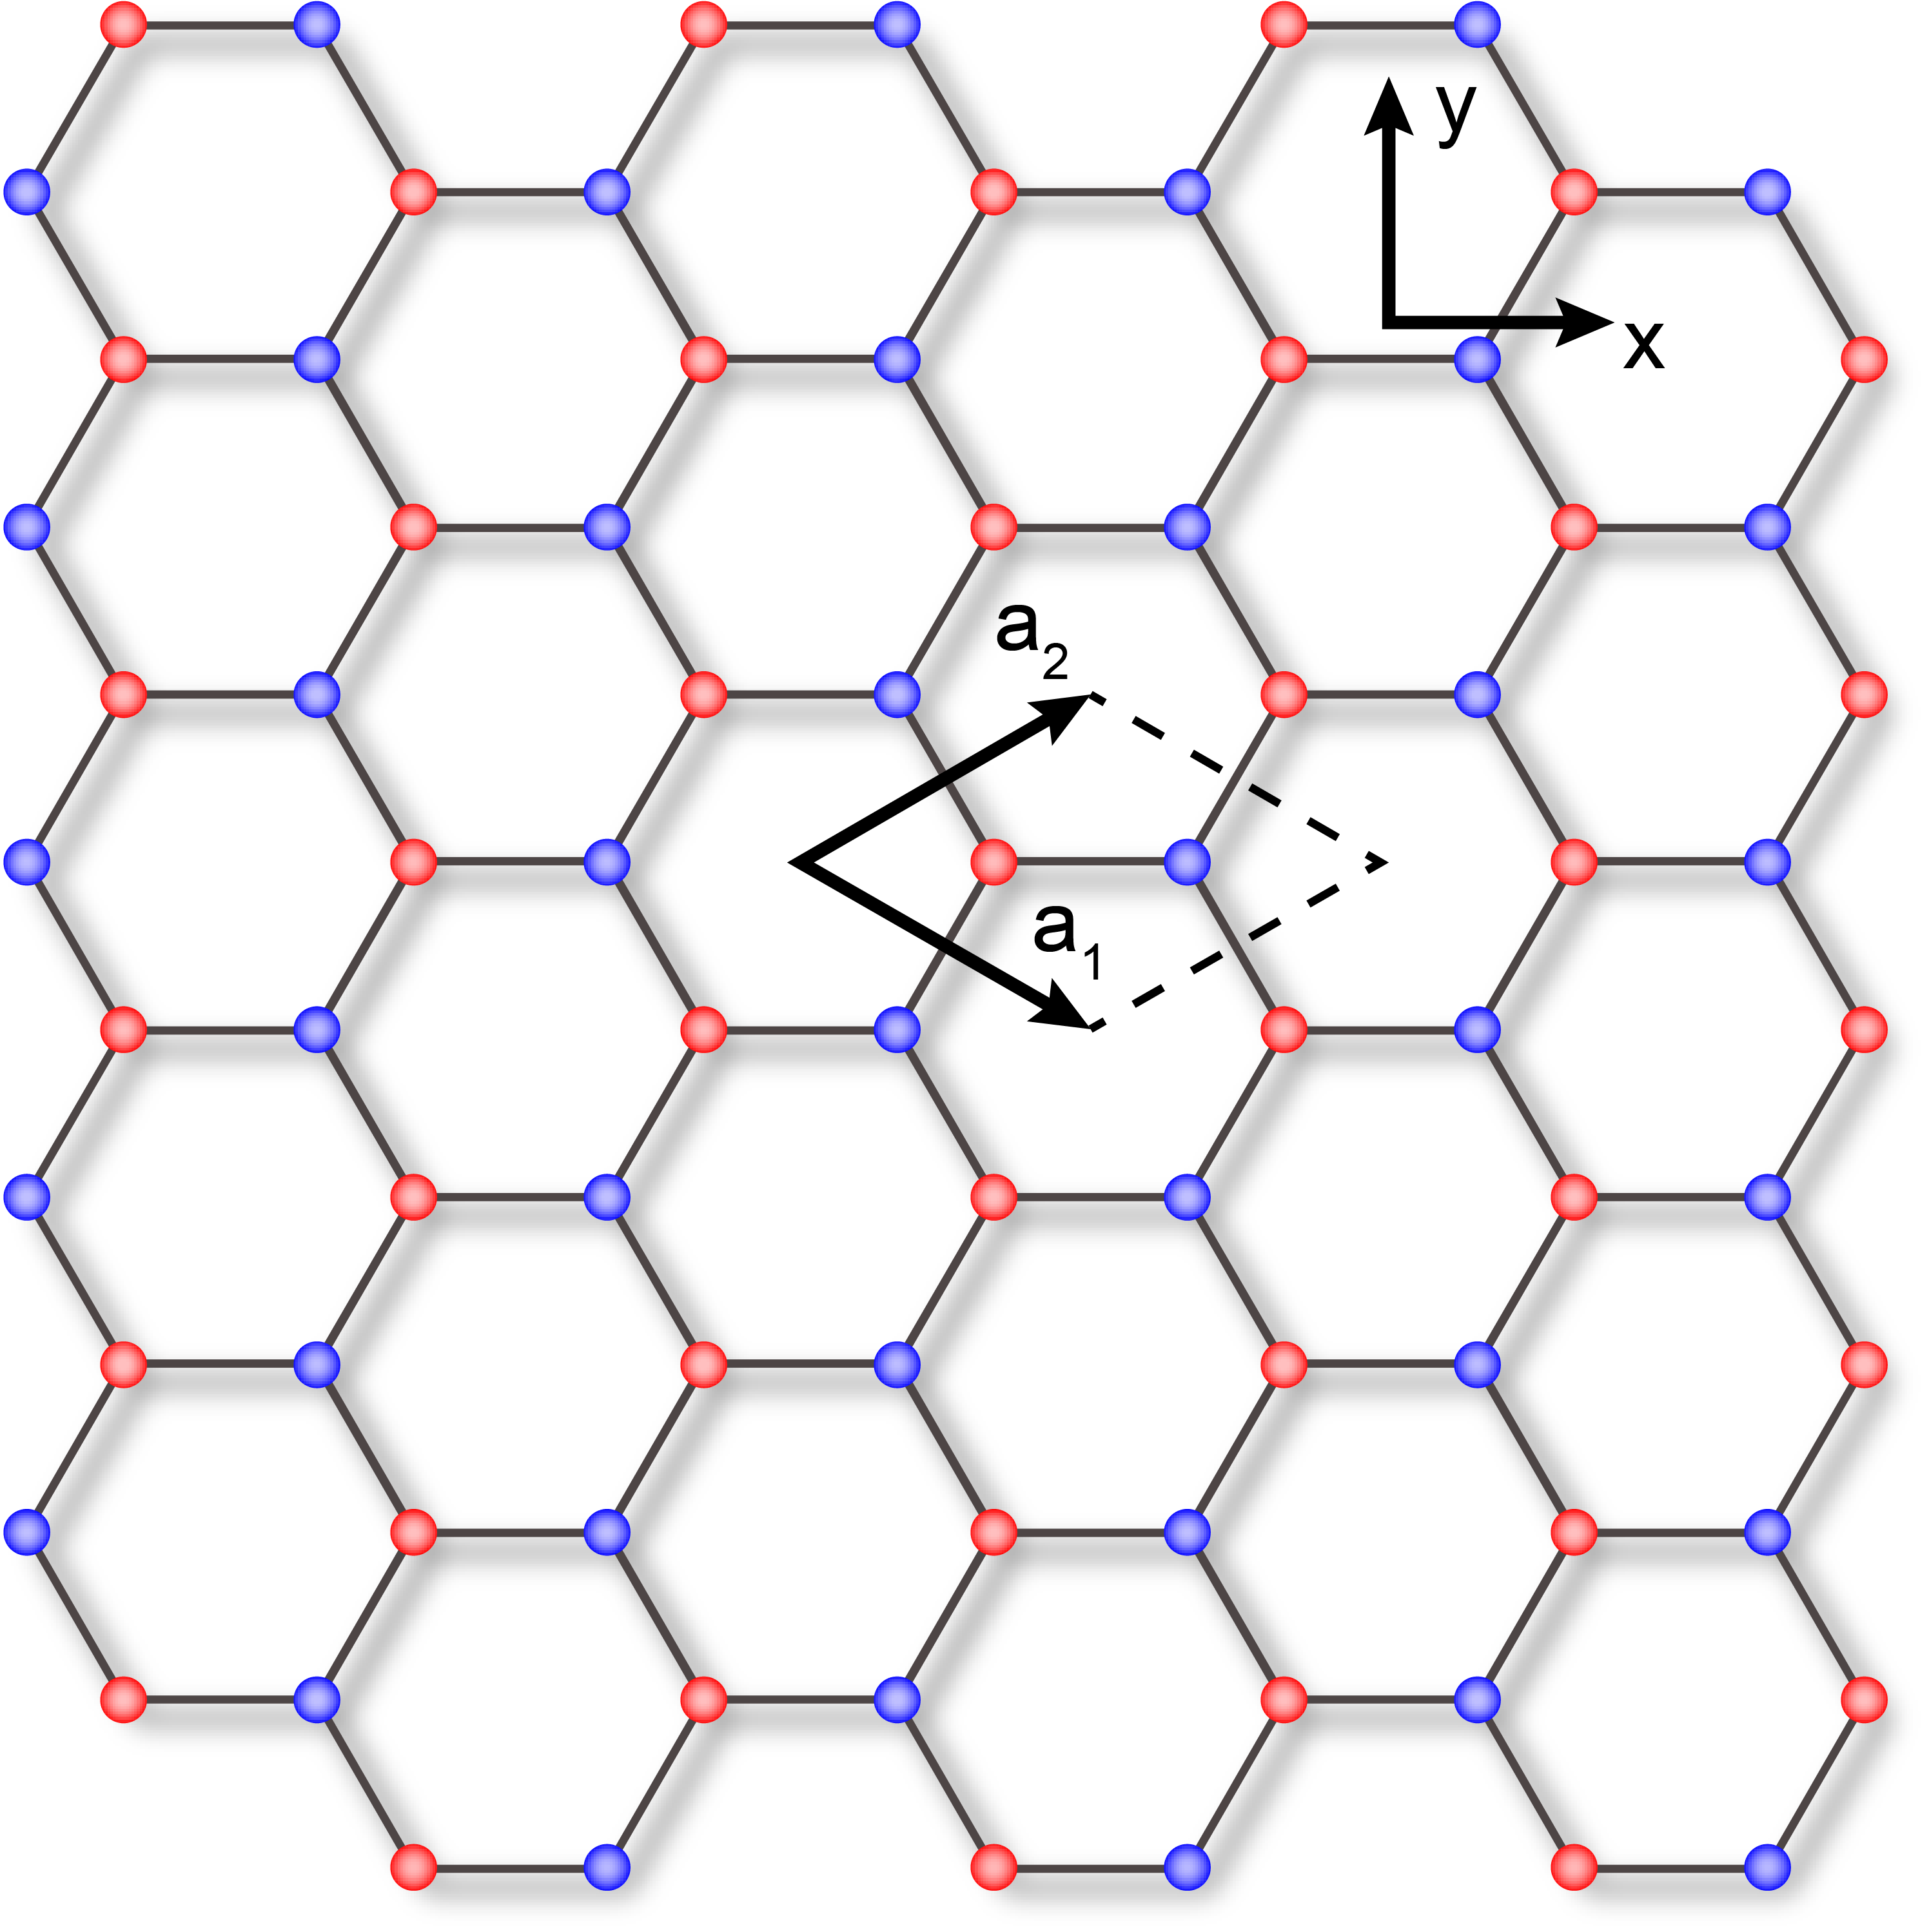
\includegraphics[width = 0.5\textwidth]{chapter2/graphene_unit_cell.png}
    \caption{The real-space structure of the graphene lattice. Vectors $\vec{a}_1$ and $\vec{a}_2$ define the unit cell, which contains two atoms, highlighted in red and blue.}
    \label{fig:graphene_unit_cell}
\end{figure}

In Figure \ref{fig:graphene_unit_cell} the unit cell is defined by the two lattice vectors $\vec{a}_1$ and $\vec{a}_2$. Each unit cell is comprised of two atoms. The honeycomb lattice can be thought of as to interpenetrating triangular sublattices. With that picture, the honeycomb unit cell contains one atom from each of the two sublattices, highlighted in Figure \ref{fig:graphene_unit_cell} as red (A) and blue (B). Each atom on the lattice contributes one conduction electron.

Using the coordinates defined in Figure \ref{fig:graphene_unit_cell}, the lattice vectors are defined, from the center of a honeycomb.

\begin{align}
    \vec{a}_1 &= \frac{3a}{2}\hat{i} + \frac{\sqrt{3}a}{2}\hat{j} \\
    \vec{a}_2 &= \frac{3a}{2}\hat{i} - \frac{\sqrt{3}a}{2}\hat{j}
\end{align}

Here $a$ is the carbon-carbon bond distance, \SI{1.42}{\angstrom} (CITE).

The reciprocal lattice vectors, $\vec{b}_1$ and $\vec{b}_2$ can now be found in the usual way.

\begin{equation}
    a_i \cdot b_j = 2\pi \delta_{ij}
\end{equation}

Here $\delta_{ij}$ is the Kronecker delta. The reciprocal lattice defined by $\vec{b}_1$ and $\vec{b}_2$ can be seen in Figure \ref{fig:graphene_k_space}.

\begin{align}
    \vec{b}_1 &= \frac{2\pi}{3a}\hat{i} + \frac{2\sqrt{3}\pi}{3a}\hat{j} \\
    \vec{b}_2 &= \frac{2\pi}{3a}\hat{i} - \frac{2\sqrt{3}\pi}{3a}\hat{j}
\end{align}

\begin{figure}
    \centering
    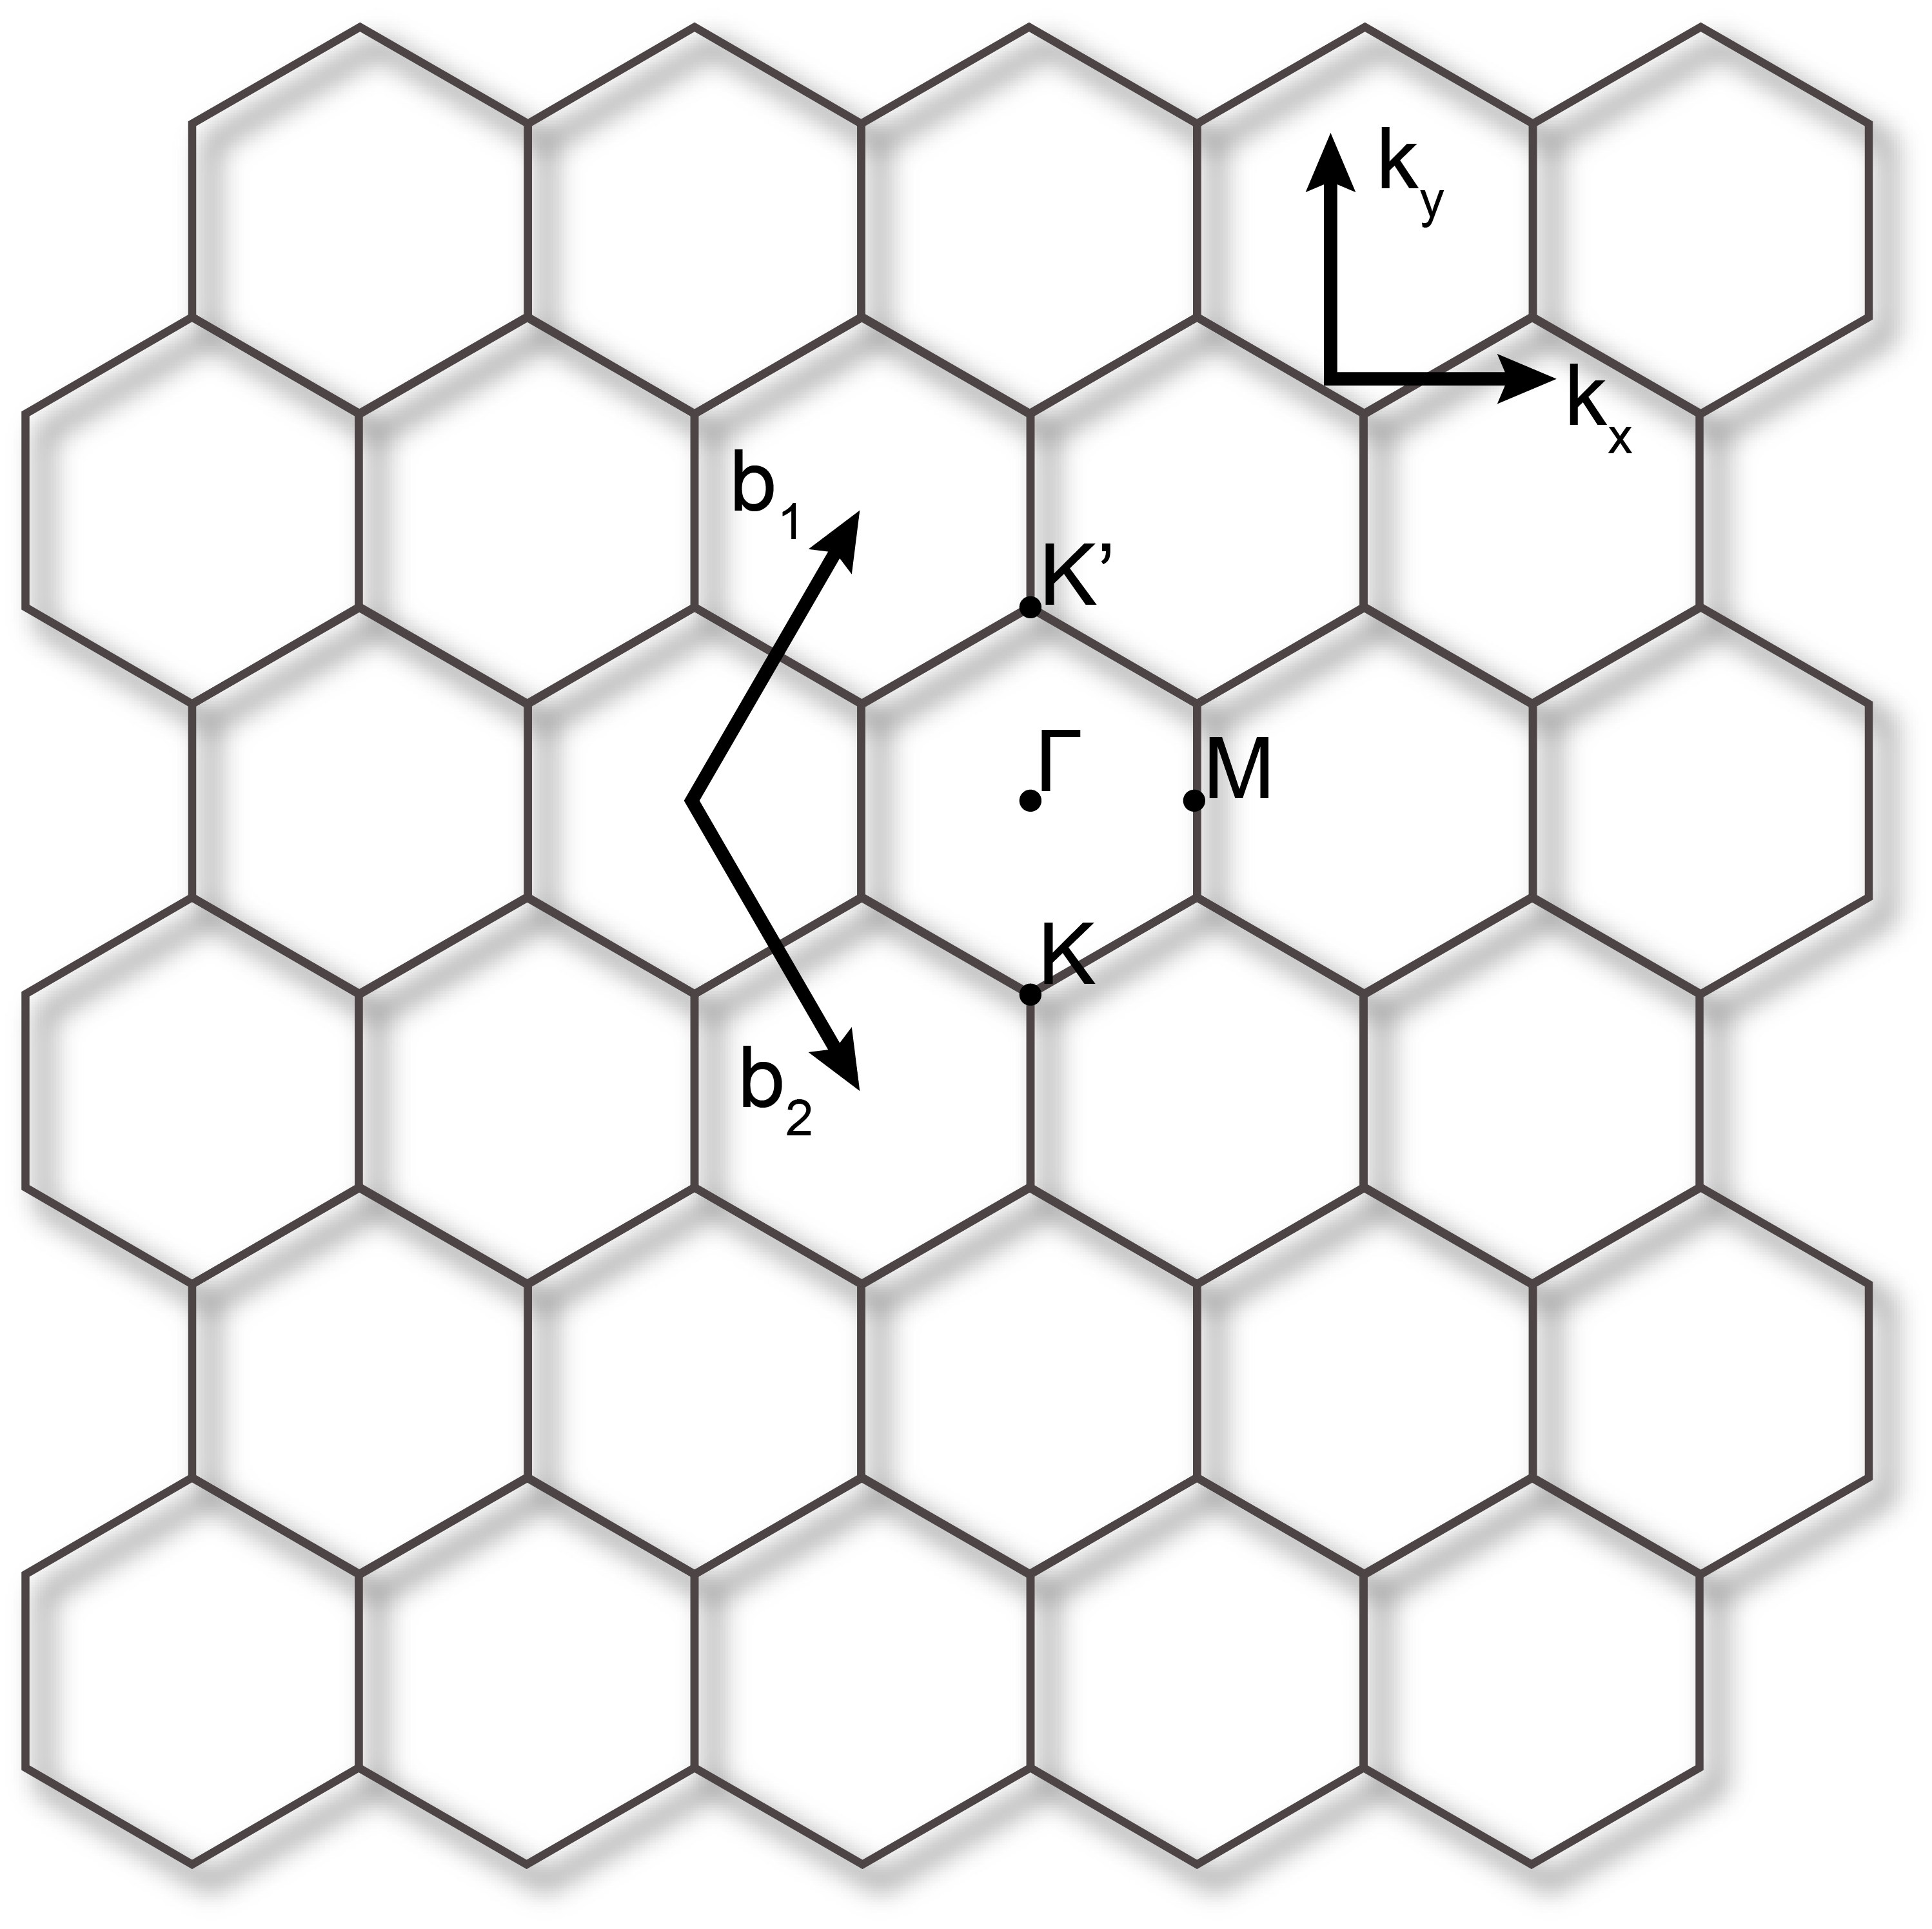
\includegraphics[width = 0.5\textwidth]{chapter2/graphene_k_space.png}
    \caption{The reciprocal lattice of graphene. Vectors $\vec{b}_1$ and $\vec{b}_2$ define the Brillouin zone. The high symmetry points $\Gamma$, $K$, $K'$, and $M$ are labeled.}
    \label{fig:graphene_k_space}
\end{figure}

The reciprocal lattice is also a honeycomb lattice, rotated 90 degrees from the real space lattice. The size of each Brillouin zone is defined by the reciprocal lattice vectors above. A few high symmetry points have been labelled in the figure. Of particular note are the three $K$ and three $K'$ points. As will be seen in the band structure calculation, these are the points at which the conduction and valence bands will meet to form the Dirac cones that give rise to graphene's interesting low energy conduction properties.

\subsection{Tight Binding Model}

The simplest way to calculate the low energy electronic band structure for graphene is using a nearest neighbor tight binding model, also known as a linear combination of atomic orbitals (CITE). In this model, each conduction electron is tightly bound to a lattice site with a small probability of hopping only to a nearest neighbor site. With this simple picture for electron conduction, one can find the lowest energy bands in graphene.

Given that the model deals with the motion of individual electrons and their wavefunctions at each atomic site, the goal will be to solve the time independent Schr\"{o}dinger equation.

\begin{equation}
    \hat{H}\Psi = \varepsilon\Psi
\end{equation}

$\Psi$ is a single particle wavefunction over the whole graphene lattice. As such, it can be written as a linear combination of Bloch wavefucntions.

\begin{align}
    u_A(\vec{r}) &= \frac{1}{\sqrt{N}}\sum_{\vec{r}_A}^{} e^{i\vec{k}\cdot\vec{r}_A} \phi_{2p_z}(\vec{r}-\vec{r}_A) \\
    u_B(\vec{r}) &= \frac{1}{\sqrt{N}}\sum_{\vec{r}_B}^{} e^{i\vec{k}\cdot\vec{r}_B} \phi_{2p_z}(\vec{r}-\vec{r}_B)
\end{align}

These two functions represent Bloch waves localized on the A and B sublattices, respectively. With these definitions the full single-particle wavefunction can be rewritten as follows:

\begin{equation}
    \Psi = C_A u_A + C_B u_B
\end{equation}

$C_{A(B)}$ represents the amplitude of the wavefunction on the A(B) sublattice. With all of the above definitions the time independent Schr\"{o}dinger equation can be rewritten in a matrix form:

\begin{equation} 
\label{eq:TISE}
    \begin{pmatrix} H_{AA} & H_{AB} \\ H_{BA} & H_{BB} \end{pmatrix} \begin{pmatrix} C_A \\ C_B \end{pmatrix} = \varepsilon \begin{pmatrix} S_{AA} & S_{AB} \\ S_{BA} & S_{BB} \end{pmatrix} \begin{pmatrix} C_A \\ C_B \end{pmatrix}
\end{equation}

Where:

\begin{align}
\label{eq:matel}
    H_{ij} &= \braket{u_i | H | u_j} \\
    S_{ij} &= \braket{u_i | u_j}
\end{align}

For simplicity, the rest of this calculation will assume $\braket{u_i | u_j} = \delta_{ij}$. Meaning, there is no overlap of the two Bloch wavefunctions and that each of the wave functions is already properly normalized. Rewriting Equation \ref{eq:TISE} yields:

\begin{equation}
\label{eq:secular}
    \begin{pmatrix} H_{AA}-\varepsilon & H_{AB} \\ H_{BA} & H_{BB}-\varepsilon \end{pmatrix} \begin{pmatrix} C_A \\ C_B \end{pmatrix} = 0
\end{equation}

Non-trival solutions to Equation \ref{eq:secular} exist only when:

\begin{equation}
\label{eq:eigenvals}
    \begin{vmatrix} H_{AA}-\varepsilon & H_{AB} \\ H_{BA} & H_{BB}-\varepsilon \end{vmatrix} = 0
\end{equation}

Solving equation \ref{eq:eigenvals} gives the energy eigenvalues in terms of the matrix elements defined in equation \ref{eq:matel}.

\begin{equation}
\label{eq:simple_bands}
    \varepsilon = H_{AA} \pm \lvert H_{AB} \rvert
\end{equation}

Where the relations $H_{AA} = H_{BB}$ and $H_{AB} = {H^*}_{BA}$ were used.

In order to obtain a useful expression for the energy bands in terms of the electron momentum $\vec{k}$, Equation \ref{eq:simple_bands} must be simplified using the expressions for the Bloch wavefunctions. 

\begin{align}
    H_{AA} &= \frac{1}{N} \sum_{\vec{r}_A}^{} \sum_{\pvec{r}'_A}^{} e^{i \vec{k}\cdot(\vec{r}_A - \pvec{r}'_A)} \int \phi^*_{2p_z}(\vec{r}-\vec{r}_A) \hat{H} \phi_{2p_z}(\vec{r}-\pvec{r}'_A) \, d^3\vec{r} \label{eq:overlap_AA} \\
    H_{AB} &= \frac{1}{N} \sum_{\vec{r}_A}^{} \sum_{\vec{r}_B}^{} e^{i \vec{k}\cdot(\vec{r}_A - \vec{r}_B)} \int \phi^*_{2p_z}(\vec{r}-\vec{r}_A) \hat{H} \phi_{2p_z}(\vec{r}-\vec{r}_B) \, d^3\vec{r} \label{eq:overlap_AB}
\end{align}

The summation in Equation \ref{eq:overlap_AA} can be evaluated to yield:

\begin{equation}
\label{eq:pz_energy}
    H_{AA} = \int \phi^*_{2p_z}(\vec{r}-\vec{r}_A) \hat{H} \phi_{2p_z}(\vec{r}-\vec{r}_A) \, d^3\vec{r} = \varepsilon_{p_z}
\end{equation}

Where $\varepsilon_{p_z}$ is the energy of a single electron on a $p_z$ orbital. For the sake of simplicity, the rest of this chapter will assume $\varepsilon_{p_z} = 0$. 

In order to simplify Equation \ref{eq:overlap_AB} it is useful to define the vectors pointing from an atom on the B sublattice to its three nearest neighbors on the A sublattice.

\begin{align}
    \vec{\delta}_1 &= -a\hat{i} \nonumber \\
    \vec{\delta}_2 &= \frac{a}{2}\hat{i} - \frac{\sqrt{3}}{2}a\hat{j} \label{eq:deltas} \\
    \vec{\delta}_3 &= \frac{a}{2}\hat{i} + \frac{\sqrt{3}}{2}a\hat{j} \nonumber 
\label{eq:deltas}
\end{align}

With these definitions Equation \ref{eq:overlap_AB} can be rewritten as:

\begin{equation}
\label{eq:AB_simple}
    \hat{H}_{AB} = \sum_{i=1}^{3} e^{i\vec{k}\cdot\vec{\delta}_i} \int \phi^*_{2p_z}(\vec{r}) \hat{H} \phi_{2p_z}(\vec{r}- \vec{\delta}_i) \, d^3\vec{r}
\end{equation}

Since the exact form of the Hamiltonian is not known, the integral in Equation \ref{eq:AB_simple} cannot be evaluated. However, the integral clearly represents the overlap between the wavefunction of an electron in a $p_z$ orbital on the A lattice and its nearest neighbor on the B lattice. With that in mind, the hopping amplitude $t$ is defined:

\begin{equation}
\label{eq:hopping_amp}
    t = \int \phi^*_{2p_z}(\vec{r}) \hat{H} \phi_{2p_z}(\vec{r}-\vec{\delta}_i) \, d^3\vec{r}
\end{equation}

Note, there is only one hopping amplitude, independent of the index $i$, since the distance between all nearest neighbors, $\lvert \delta_i \rvert$, is the same. With this definition, the overlap integral can be rewritten once more.

\begin{equation}
\label{eq:AB_final}
    H_{AB} = t \sum_{i=1}^{3} e^{i\vec{k}\cdot\vec{\delta}_i}
\end{equation}

Equation \ref{eq:AB_final} can be combined with the assumption that the onsite energy can be set to zero, $\varepsilon_{p_z} = 0$ to give the final effective Hamiltonian for this model.

\begin{equation}
\label{eq:effective_H}
    \hat{H} = \begin{pmatrix} 0 & t \sum_{i}^{} e^{i\vec{k}\cdot\vec{\delta}_i} \\  t \sum_{i}^{} e^{-i\vec{k}\cdot\vec{\delta}_i} & 0 \end{pmatrix}
\end{equation}

Using these same results in Equation \ref{eq:simple_bands} gives the two lowest energy bands in terms of the hopping amplitude, $t$. 

\begin{equation}
    \varepsilon(\vec{k}) = \pm t \left| \sum_{i}^{} e^{i \vec{k}\cdot\vec{\delta}_i} \right|
    \label{eq:f_k}
\end{equation}

\begin{equation}
    \varepsilon(\vec{k}) = \pm t \sqrt{ 1 + 4\cos\left(\frac{3a}{2}k_x\right)\cos\left(\frac{\sqrt{3}a}{2}k_y\right) + 4\cos^{2}\left(\frac{\sqrt{3}a}{2}k_y\right)} \label{eq:bands}
\end{equation}    

These two bands can be seen in Figure \ref{fig:graphene_bands}. Note that the plot does not assume  $S_{ij} = \braket{u_i | u_j} = \delta_{ij}$, which introduces some asymmetry in the valence and conduction bands.

\begin{figure}
    \centering
    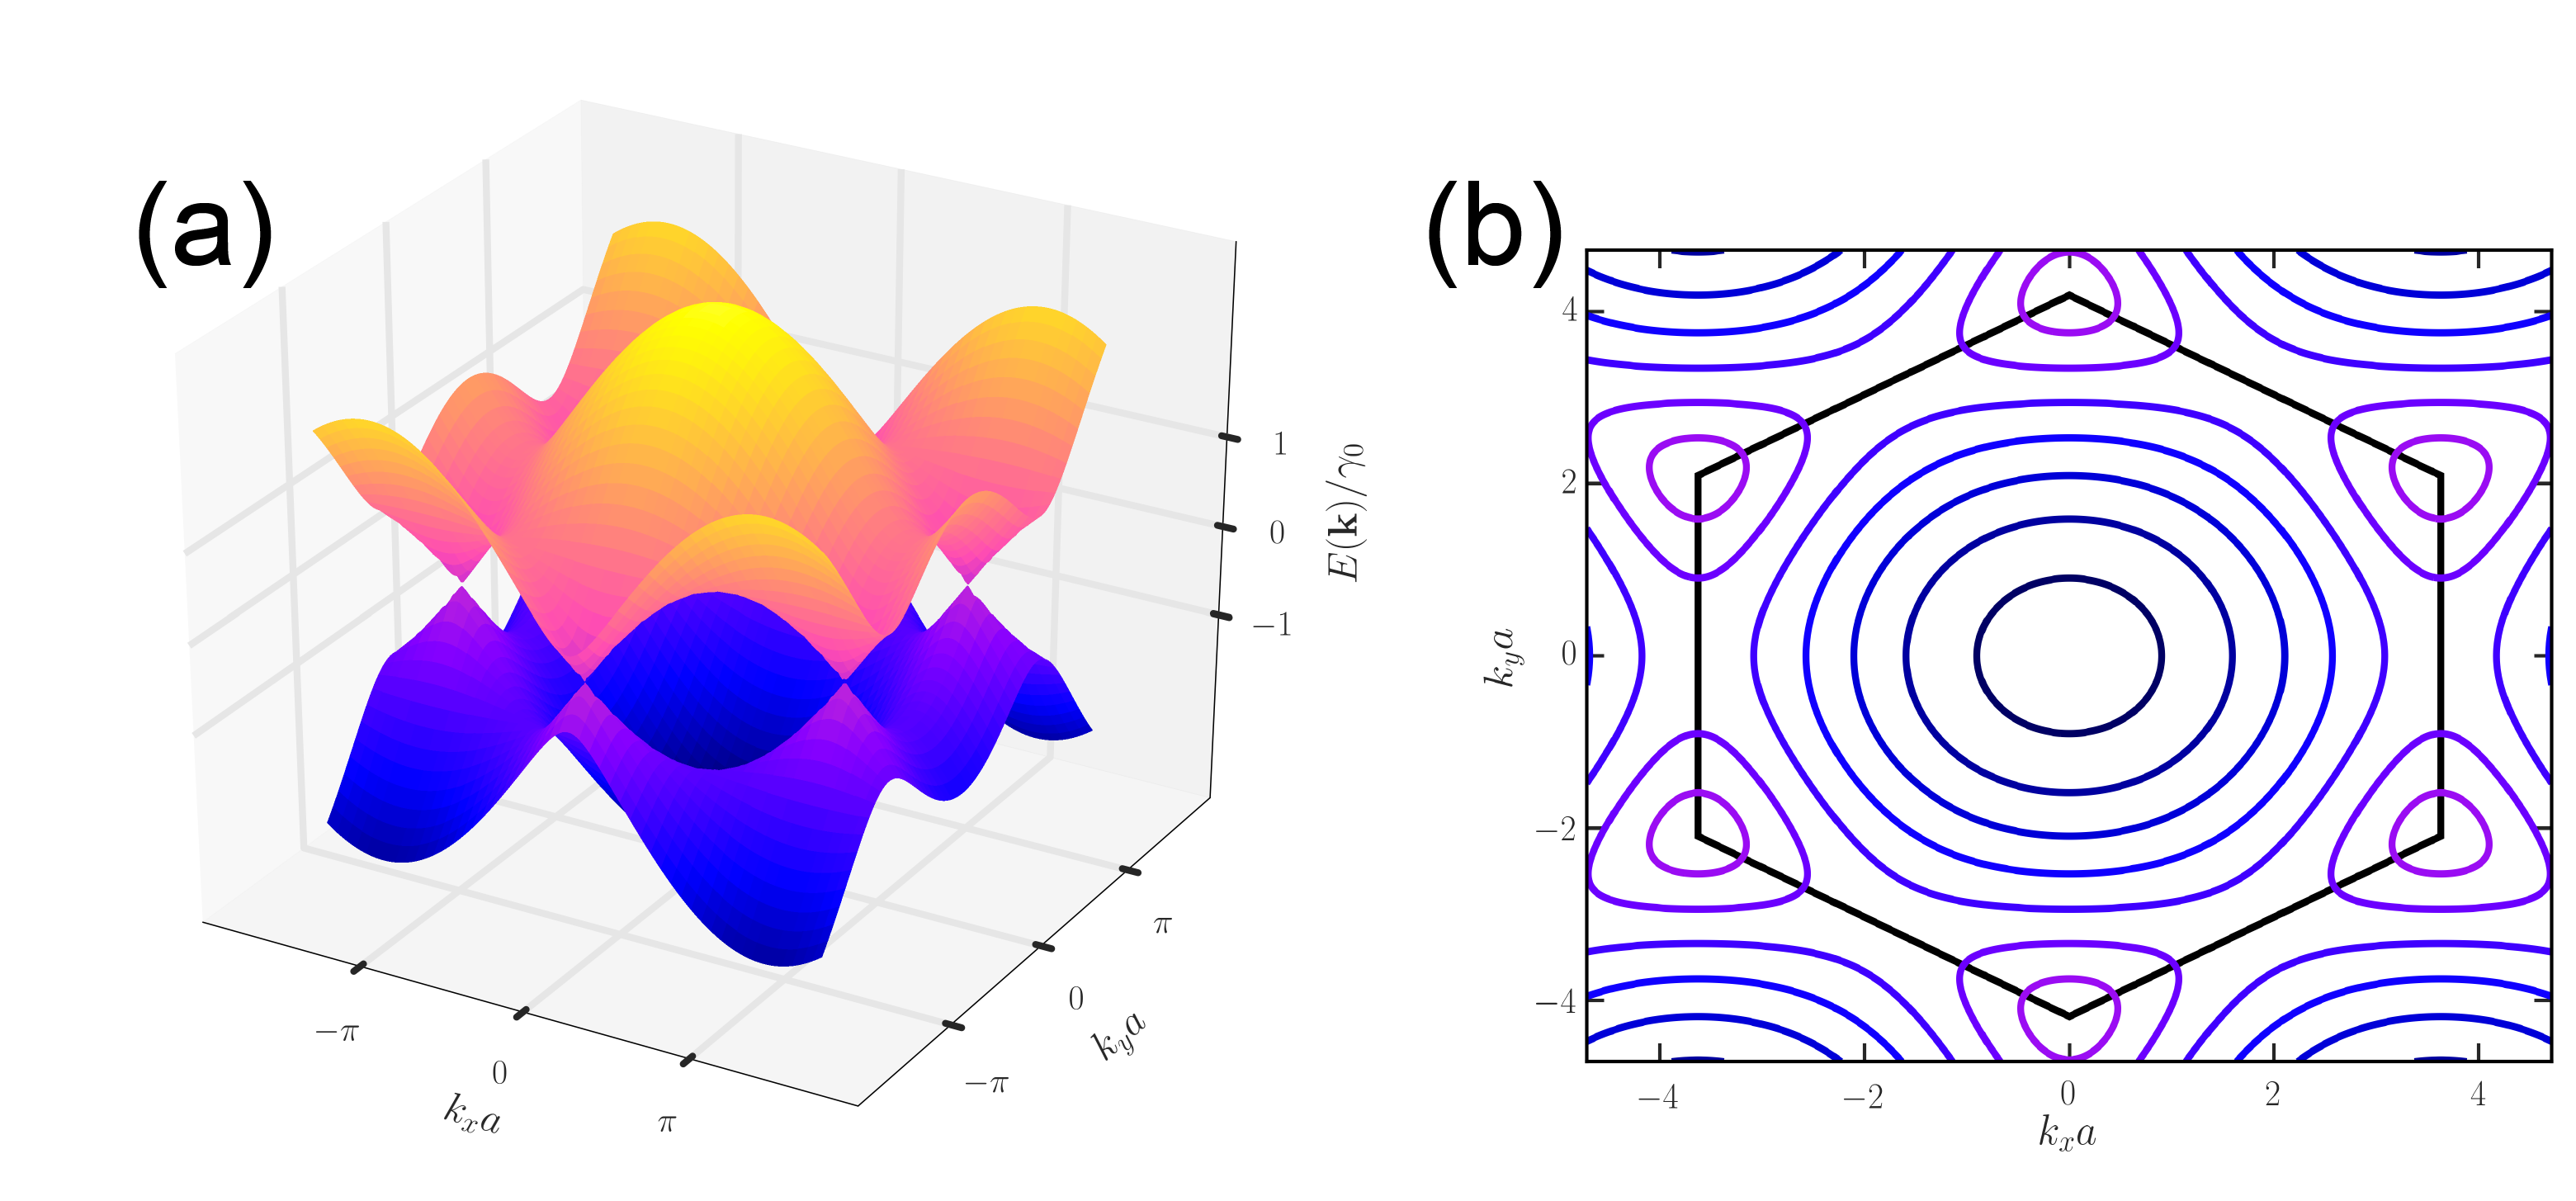
\includegraphics[width = 1.0\textwidth]{chapter2/graphene_band_fig.png}
    \caption{(a) The $\pi$-bands of graphene calculated using a nearest neighbor tight binding model. (b) A contour plot of the upper band with the first Brillouin zone drawn. The bands meet at the three $K$ and three $K'$ points at the vertices of the Brillouin zone.}
    \label{fig:graphene_bands}
\end{figure}

\subsection{Low Energy Bandstructure of Graphene}

For low energy electronic excitations, conduction will be dominated by the bandstructure near the $K$ and $K'$ points. There are only two inequivalent points, since the other 4 are equivalent by the symmetry of the honeycomb lattice. Consider the two points located at:

\begin{align}
    \vec{K} &= 0\hat{i} - \frac{4\pi}{3\sqrt{3}a}\hat{j} \\
    \pvec{K}' &= -\vec{K} = 0\hat{i} + \frac{4\pi}{3\sqrt{3}a}\hat{j}
\end{align}

To get the low-energy dispersion relation, expand the Hamiltonian in Equation \ref{eq:effective_H} around the $K$ point.

\begin{equation}
    \vec{k} = \vec{K} + \vec{q}
\end{equation}

\begin{equation}
\label{eq:approx_HK}
    \hat{H} \approx -i\frac{3at}{2} \begin{pmatrix} 0 & q_x+iq_y\\ -(q_x-iq_y)& 0 \end{pmatrix}
\end{equation}

Similarly, expanding around the $K'$ point yields:

\begin{equation}
\label{eq:approx_HKp}
    \hat{H} \approx -i\frac{3at}{2} \begin{pmatrix} 0 & q_x-iq_y\\ -(q_x+iq_y)& 0 \end{pmatrix}
\end{equation}

By defining $v_f \equiv {3at}/{2\hbar}$, using the standard Pauli matrices, and rotating the phase, Equations \ref{eq:approx_HK} and \ref{eq:approx_HKp} can be written in a more suggestive form. 

\begin{align}
    \hat{H}_K &= \hbar v_f \vec{\sigma}\cdot\vec{q} \label{eq:chiral_HK} \\
    \hat{H}_{K'} &= \hbar v_f \pvec{\sigma}^*\cdot\vec{q} \nonumber
\end{align}

These Hamiltonians describe massless Dirac fermions in 2D. This is clear in the low-energy dispersion relation.

\begin{equation}
\label{eq:massless_disp}
    \varepsilon(\vec{q}) = \pm\hbar v_f q
\end{equation}

It is also important to note, in Equation \ref{eq:chiral_HK}, that the sublattice structure has lead to a spin-1/2 degree of freedom. This degree of freedom is known as the valley degeneracy or pseudospin. 

A useful consequence of the pseudospin is the reduction in scattering in graphene and carbon nanotubes. The reduced backscattering is a result of the introduction of an additional symmetry to the system. This reduction in scattering leads to unusually high mobilities and long spin coherence lengths in both materials. The increased spin coherence length is exactly what lead to the choice of carbon nanotubes for this work.

\section{Electronic Bandstructure of Carbon Nanotubes} 

Now that the bandstructure a graphene sheet has been calculated, finding the electronic bandstructure of various carbon nanotubes is as simple as applying a few boundary conditions.

The structure of a carbon nanotube can be completely described by its chiral vector.

\begin{align}
    \vec{C}_h &= m\vec{a}_1 + n\vec{a}_2 \label{eq:chiral_vec} \\
    \vec{C}_h &= \frac{3}{2}(n+m)a\hat{i} + \frac{\sqrt{3}}{2}(n-m)a\hat{j} \nonumber
\end{align}

This vector describes how to roll a graphene sheet to form the nanotube. The tube is formed by rolling the graphene sheet such that the tip and tail of $\vec{C}_h$ meet. The indices $(n,m)$ describe the type of nanotube that is formed. A tube where $0<m<n$ is known as chiral, $m=n$ is an armchair nanotube, and $m=0$ is a zig-zag nanotube. Armchair and zig-zag tubes get their names from the shape of the carbon bonds on the edge of the unit cell.

\begin{figure}
    \centering
    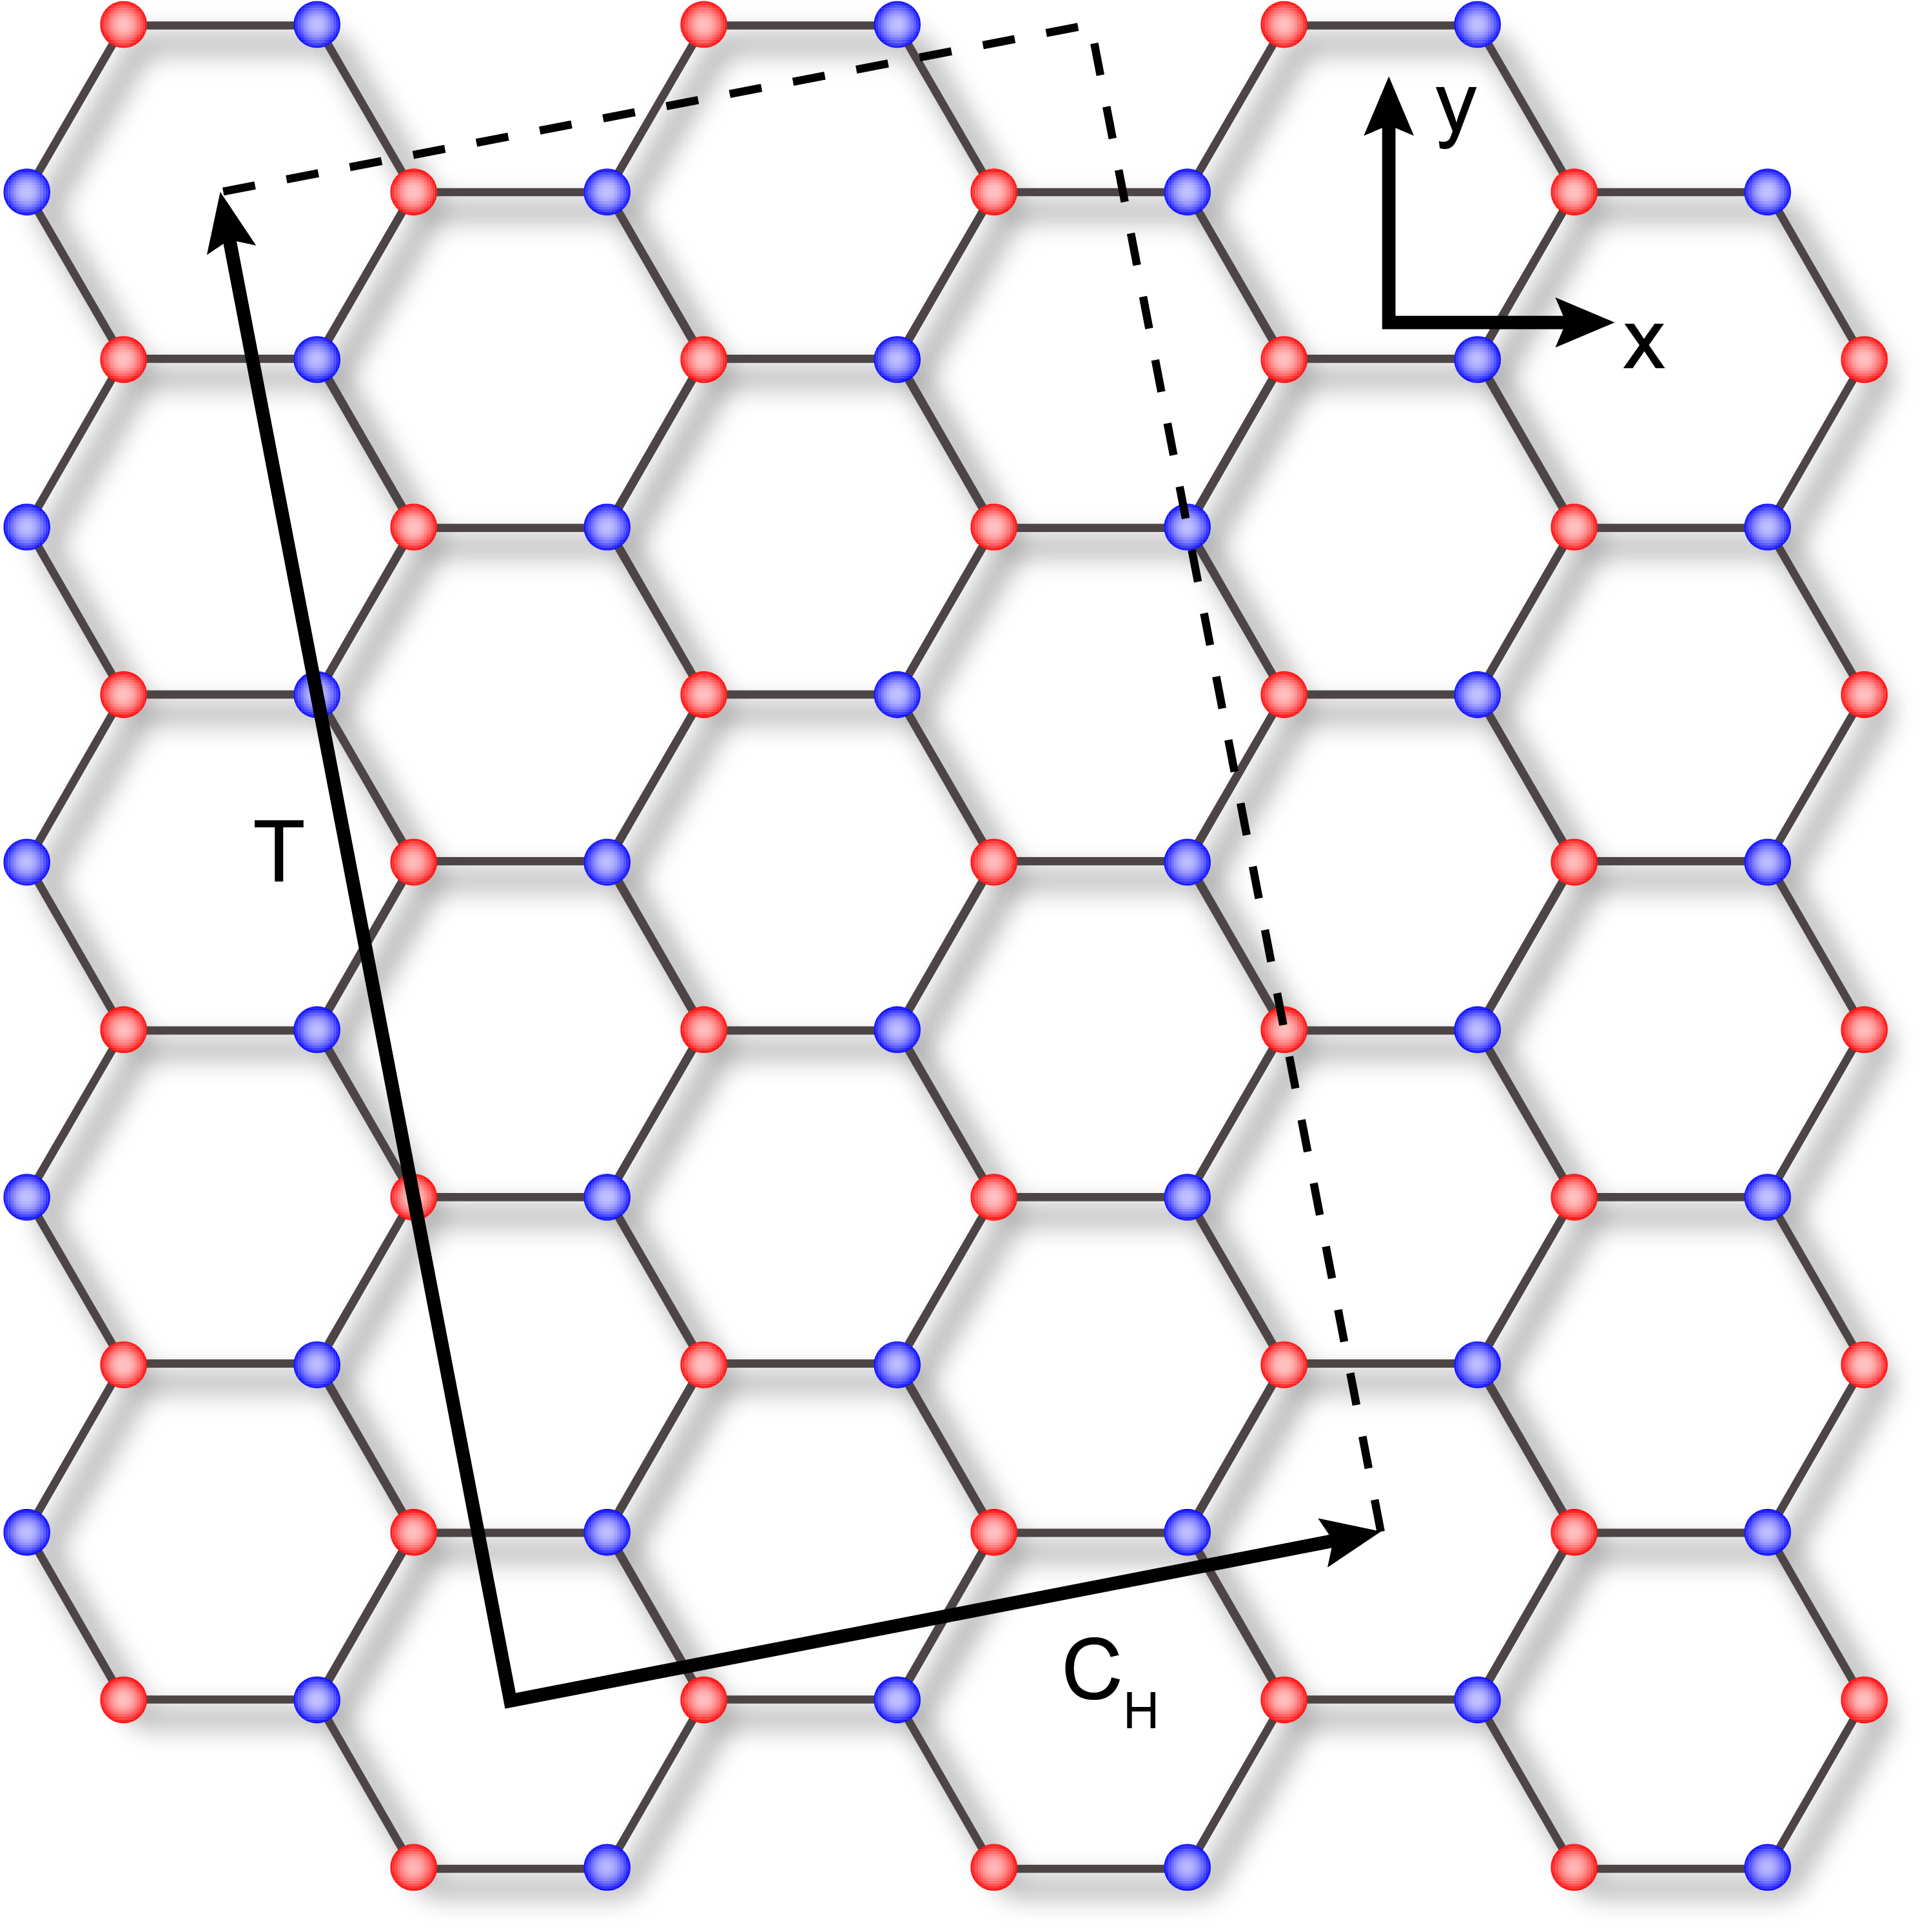
\includegraphics[width = 0.5\textwidth]{chapter2/nanotube_unit_cell.png}
    \caption{The real-space structure of a carbon nanotube. The nanotube unit cell is defined by the vectors $\vec{C}_h$ and $\vec{T}$}
    \label{fig:cnt_unit_cell}
\end{figure}

An example of a chiral (2,1) nanotube unit cell can be seen in Figure \ref{fig:cnt_unit_cell}. The unit cell is defined by the chiral vector $\vec{C_h}$ and the translation vector $T$. Which is defined as:

\begin{equation}
    \vec{T} = t_1\vec{a}_1 + t_2\vec{a}_2 \label{eq:translation}
\end{equation}
    
where $t_1 = (2m+n)/d_R, t_2 = (2n-m)/d_R$ and $d_R = gcd(2n+m, 2m+n)$ These two vectors can be used to calculate a few basic properties of the nanotube. The diameter of the nanotube is found from the chiral vector.

\begin{equation}
    d = \left| \vec{C}_h \right|/\pi = \frac{\sqrt{3}a}{\pi}\sqrt{n^2+nm+m^2}
    \label{eq:cnt_diameter}
\end{equation}

The number of graphene unit cells contained in the nanotube unit cell is also easily calculated.

\begin{equation}
    N = \frac{\left| \vec{C}_h \times \vec{T} \right|}{\left| \vec{a}_1 \times \vec{a}_2 \right|} = \frac{2}{d_R}\sqrt{n^2+nm+m^2}
    \label{eq:cnt_N}
\end{equation}

Knowing the number of graphene unit cells contained in the nanotube unit cell yields a lot of useful information about the band structure. There are 2N carbon atoms in the nanotube unit cell and N conduction electrons. There will be 2N bands (one for each carbon atom) that will be half-filled, just like the graphene bandstructure.

The reciprocal lattice vectors for the carbon nanotube defined by $(n,m)$ can be found in the usual way.

\begin{align}
    \vec{C}_h\cdot\vec{K}_1 &= \vec{T}\cdot\vec{K}_2 = 2\pi \nonumber \\
    \vec{C}_h\cdot\vec{K}_2 &= \vec{T}\cdot\vec{K}_1 = 0 \label{eq:cnt_recip}
\end{align}
    
\begin{align}
    \vec{K}_1 &= -\frac{(t_2 \vec{b}_1 - t_1 \vec{b}_2)}{N} \nonumber \\
    \vec{K}_2 &= \frac{(m \vec{b}_1 - n \vec{b}_2)}{N} \label{eq:K1_K2}
\end{align}

The reciprocal space of the unrolled nanotube is quantized along $\vec{K}_1$ and continuous along $\vec{K}_2$. This means the electron momentum $k$ in the nanotube is quantized along the direction of $C_h$. These quantized 'cutting lines' define the electronic bands in the carbon nanotube.

\begin{equation}
    \vec{k}\cdot\vec{C}_h = 2\pi\mu
\end{equation}

Where $\mu$ is an integer from $1-N/2$ to $N/2$ and $\mu=0$ cuts through the $\Gamma$ point at the center of the graphene Brillouin zone. The structure of the nanotube reciprocal lattice, definied by $K_1$ and $K_2$ can be seen in Figure \ref{fig:cnt_k_space}. 

\begin{figure}
    \centering
    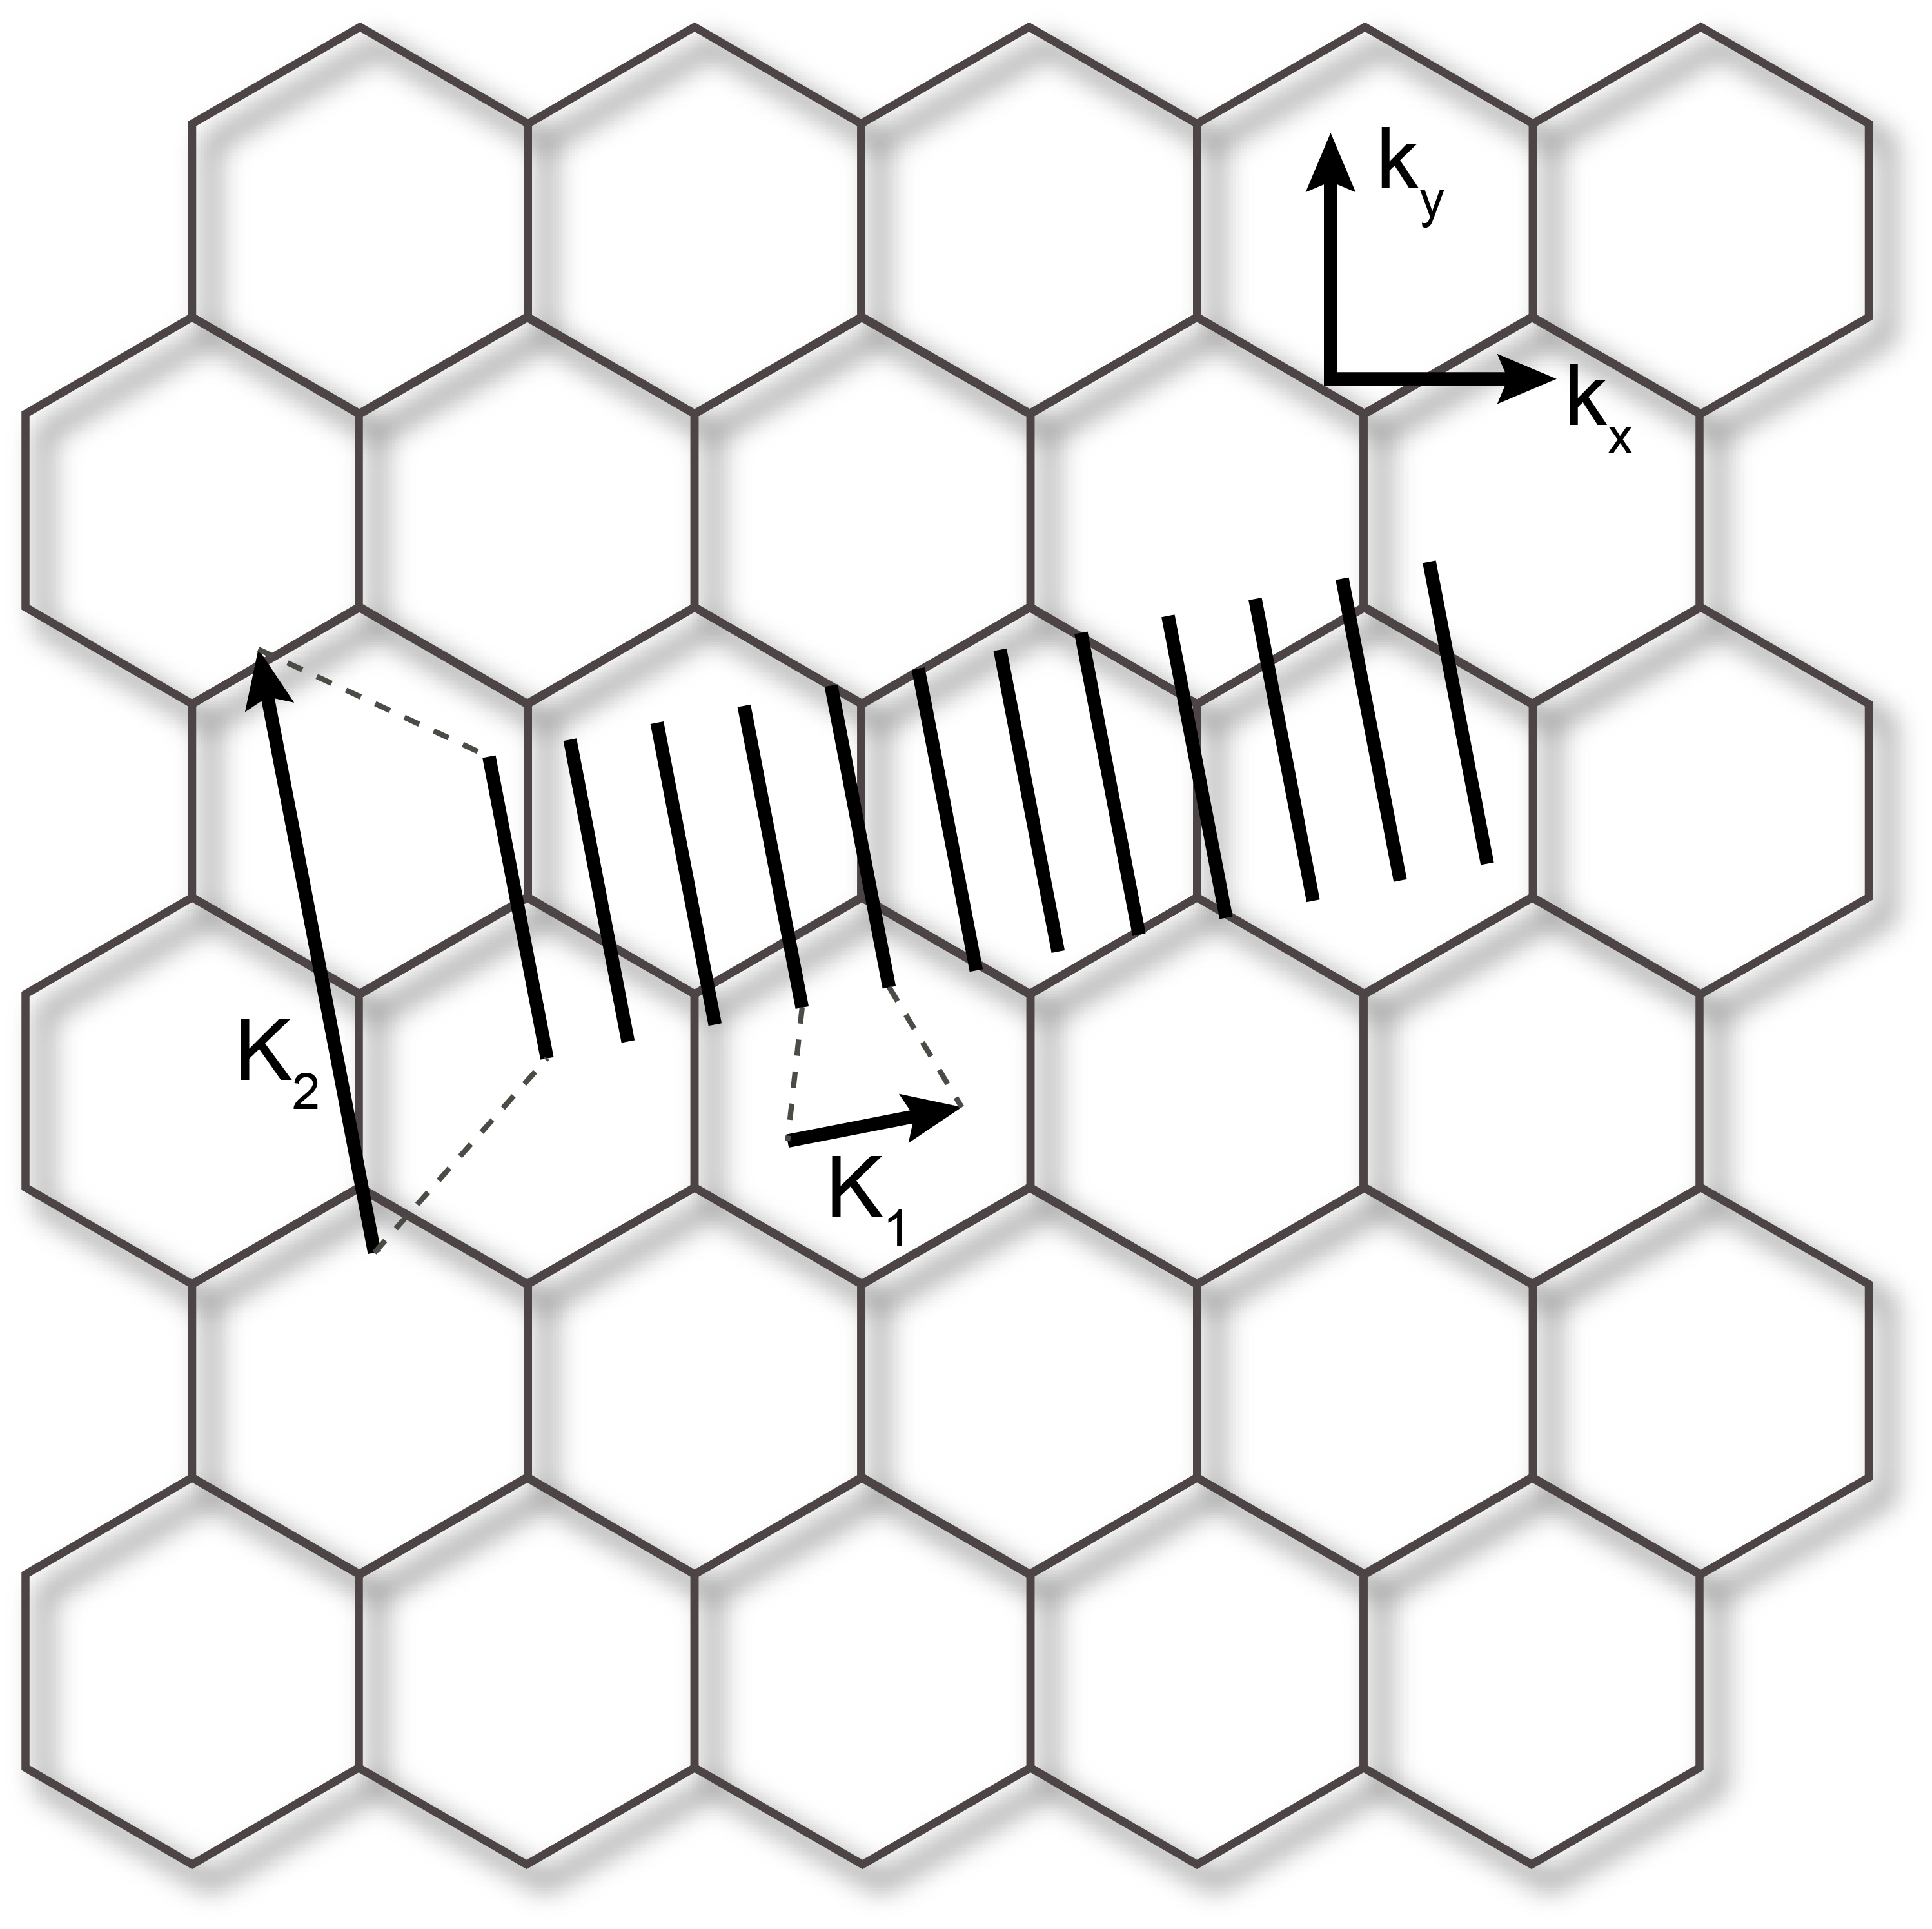
\includegraphics[width = 0.5\textwidth]{chapter2/nanotube_k_space.png}
    \caption{The reciprocal lattice of a carbon nanotube, defined by the vectors $K_1$ and $K_2$}
    \label{fig:cnt_k_space}
\end{figure}

With all of these definitions, the electron momentum in the carbon nanotube can be rewritten.

\begin{equation}
    \vec{k} = \mu\vec{K}_1 + k_{\parallel}\frac{\vec{K}_2}{|\vec{K}_2|}
    \label{eq:k_quant}
\end{equation}

The bands for a generic nanotube can be found by simply inserting this definition for the momentum into the graphene bands derived in Equation \ref{eq:bands}. 

\subsection{Types of Carbon Nanotubes}

The electronic properties of a carbon nanotube are determined by its chirality, $(n,m)$. If one of the cutting lines, as seen in Figure \ref{fig:cnt_k_space}, passes through a $K$ or $K'$ point, the nanotube will have a metallic band structure. Like in graphene, two of the valence and conduction bands will meet at discrete points at the Fermi energy. If this is not the case, and none of the cutting lines pass through a $K$ or $K'$ point, the nanotube will be semiconducting with a bandgap determined by the chirality.

To determine if a nanotube is semiconducting or metallic, one can look at the projection of $\vec{K}$, the vector pointing to a $K$ point in the graphene Brillouin zone, and $\vec{K}_1$, the nanotube reciprocal lattice vector.

\begin{equation}
    \frac{\vec{K}\cdot\vec{K}_1}{\vec{K}_1\vec{K}_1} = \frac{(2n+m)}{3} 
    \label{eq:metallic_condition}
\end{equation}

From Equation \ref{eq:metallic_condition}, it is clear that a nanotube is metallic if $(n-m)\bmod3 = 0$. There are two other cases, where $(n-m)\bmod3 = 1$ or $(n-m)\bmod3 = 2$. Each of these results in a semiconducting nanotube. Based on these results, in a collection of nanotubes with random chirality, $(n,m)$, there will be roughly $1/3$ metallic and $2/3$ semiconducting nanotubes.

Figure \ref{fig:cnt_types} shows the full bandstructure of a metallic $(5,5)$ armchair nanotube and a semiconducting $(4,2)$ chiral nanotube. These have 20 and 56 bands, respectively.

\begin{figure}
    \centering
    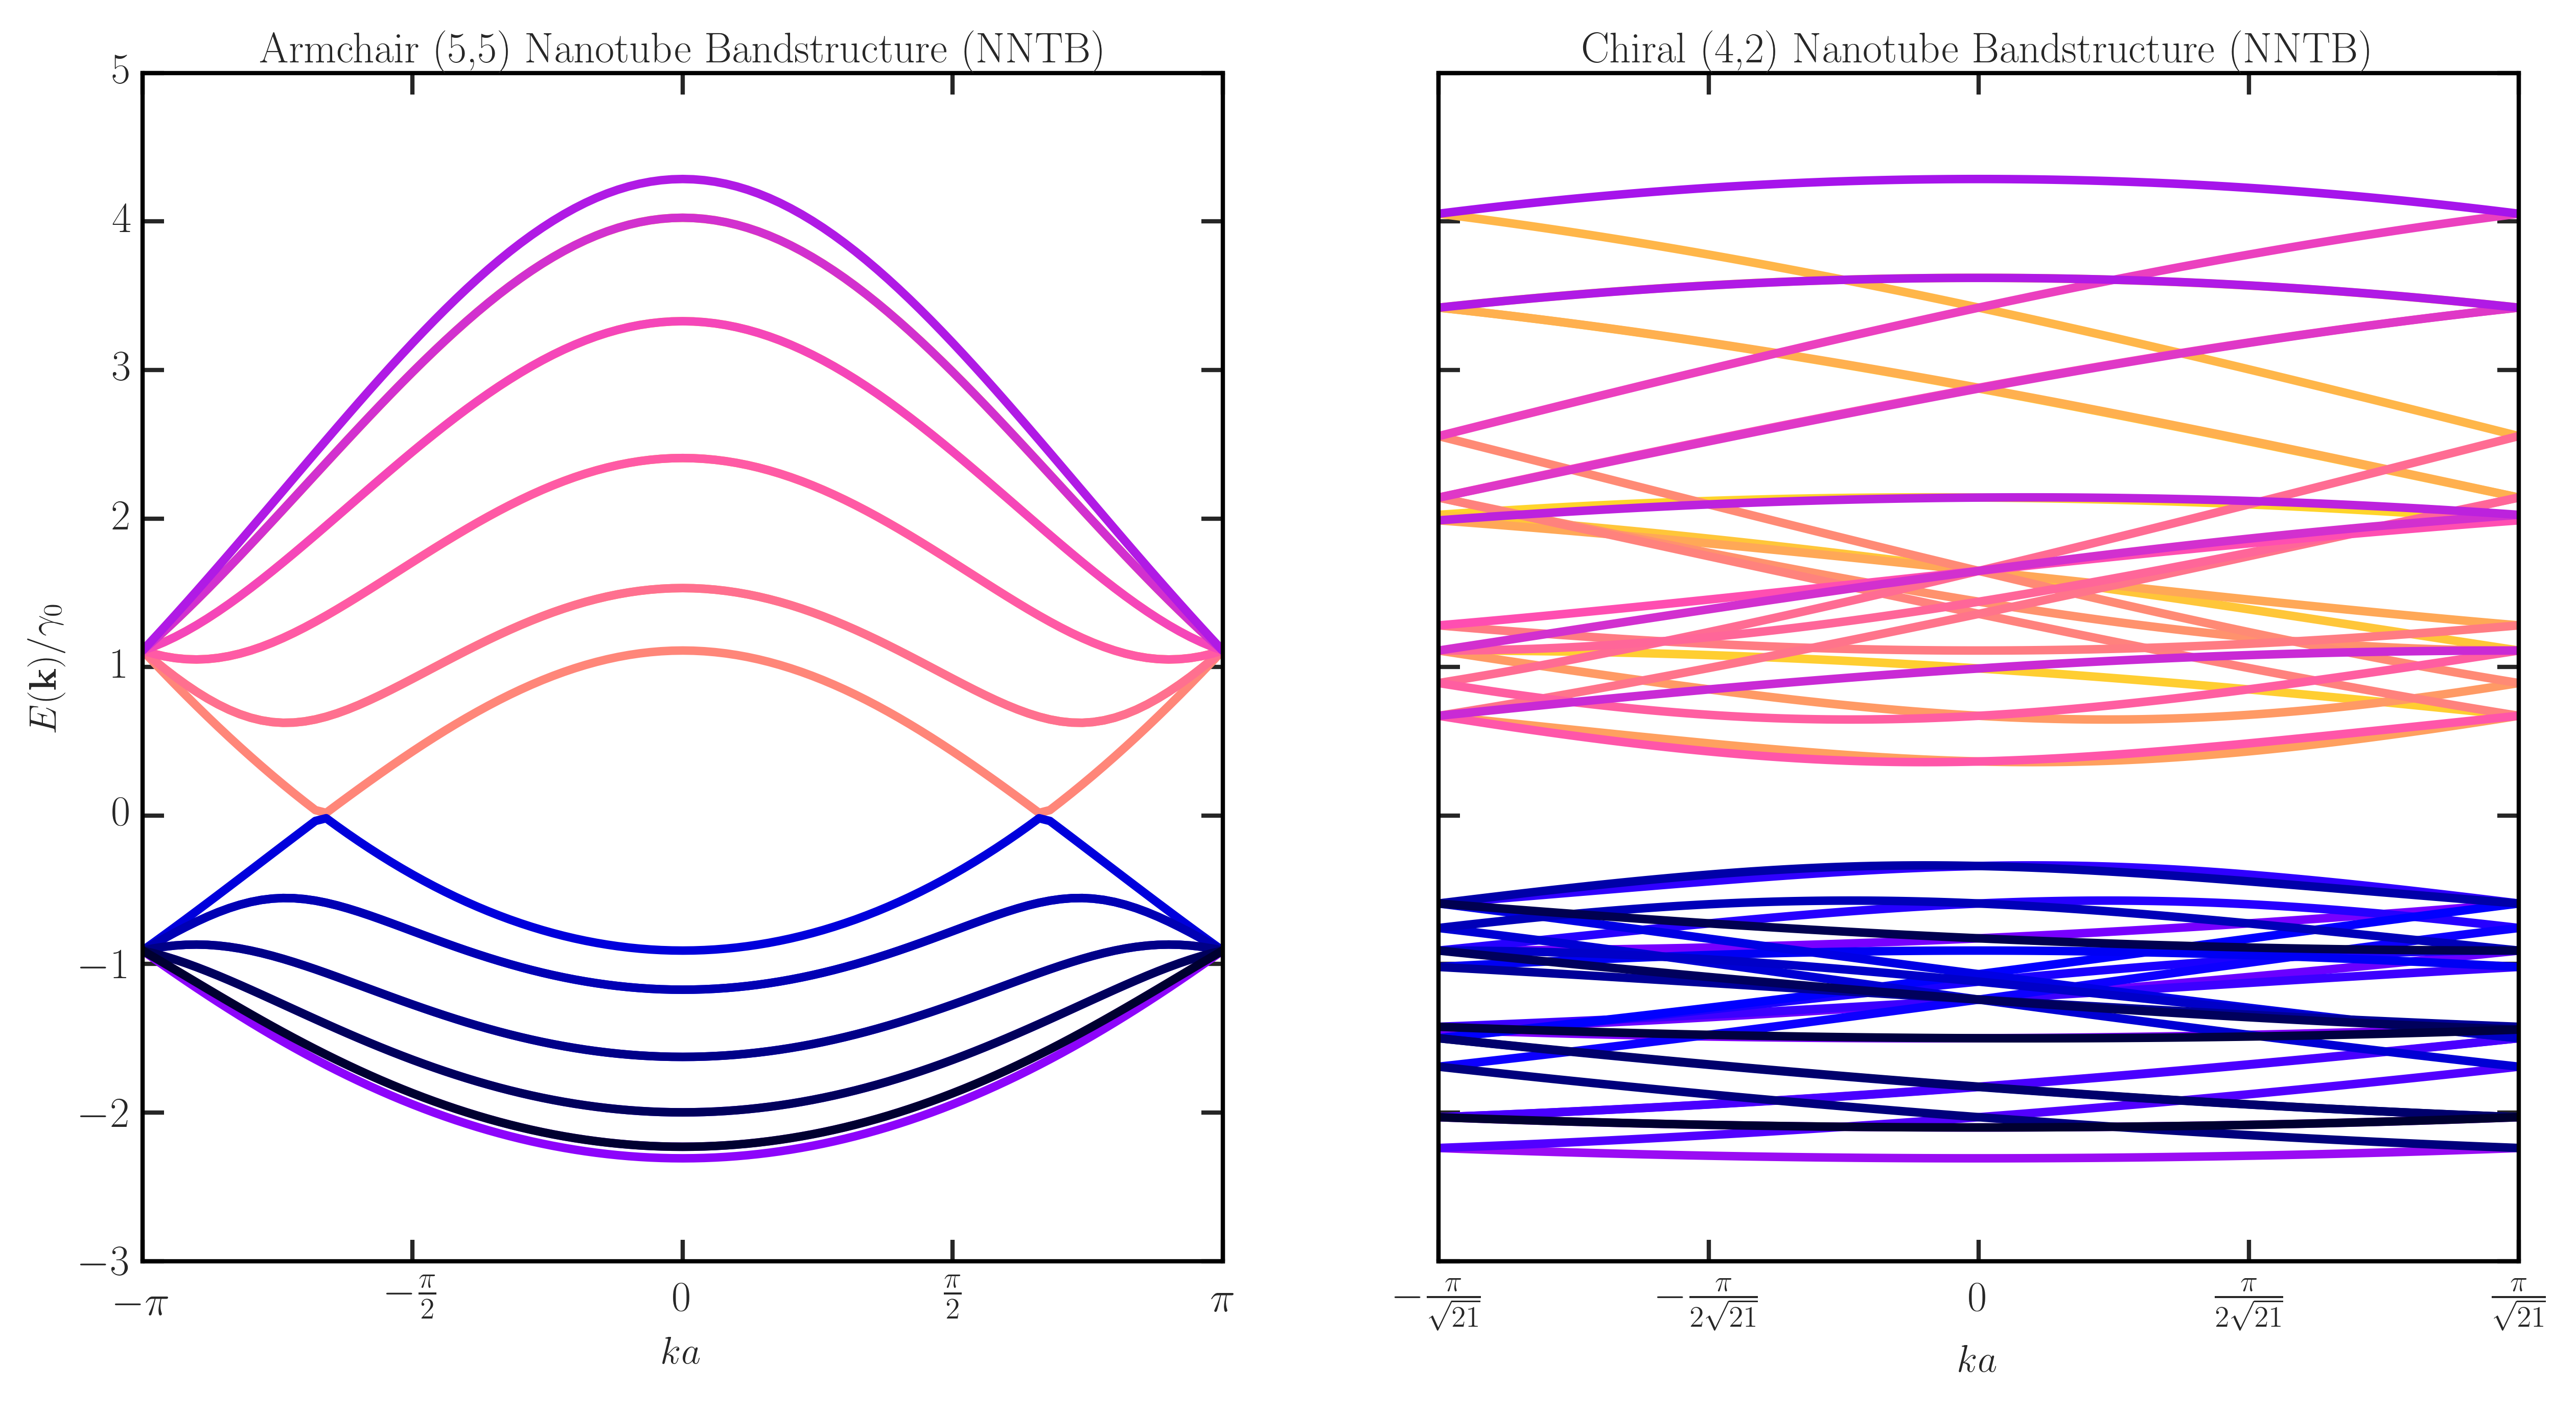
\includegraphics[width = 1.0\textwidth]{chapter2/cnt_types.png}
    \caption{Two types of carbon nanotube bandstructure. The left plot shows a metallic $(5,5)$ armchair nanotube. The right plot shows a semiconducting $(4,2)$ chiral nanotube.}
    \label{fig:cnt_types}
\end{figure}


\subsection{Low Energy Bandstructure of Carbon Nanotubes}

To calculate the full set of bands for a generic nanotube $(n,m)$ is cumbersome. The basic proprties for a generic nanotube can be more easily calculated by first expanding the graphene bands about the $K$ and $K'$ points as in Equation \ref{eq:massless_disp}, then using the quantized momentum derived in Equation \ref{eq:k_quant}. Doing this yields the low energy dispersion relation for a generic carbon nanotube.

\begin{equation}
    \varepsilon_{\mu}(k) = \pm\frac{2\hbar v_f}{d}\sqrt{\left(\frac{m-n}{3} - \mu\right)^2 + \left(\frac{kd}{2}\right)^2}
    \label{eq:low_e_cnt}
\end{equation}

Where $\mu$ is the band index, $d$ is the nanotube diameter, and k is the electron momentum along the nanotube axis. Looking at the first term in parentheses, it is clear that the nanotube will be metallic if $(m-n)/3$ is an integer. In that case, there will be some integer $\mu$ for which the valence and conduction bands meet at the Fermi energy. This is consistent with the condition derived previously for metallic and semiconducting chiral vectors. Using that information the low energy bandstructure can be written a little more suggestively.

\begin{align}
    \varepsilon(k) &= \pm\left(\frac{1}{2}E_g(n,m) + \frac{\hbar^2}{2m^*}k^2\right) \\
    \varepsilon(k) &= \pm\hbar v_f k
\end{align}

These are the approximate bandstructures at low energy. Semiconducting nanotubes have a bandgap, $E_g(n,m)$ dependent on the chirality, and an effective mass $m^*$ dependent on the lowest band curvature. Metallic nanotubes maintain the massless Dirac fermion properties found in graphene at low energies.

\section{Carbon Nanotube Field Effect Transistors}

Now that the electronic bandstructure of a carbon nanotube is known, we can move on to discussing electric measurements on simple carbon nanotube devices. At room temperature, the simplest device that one can make with a carbon nanotube is a field effect transistor. A nanotube is placed, or grown, on a silicon substrate capped with an insulating silicon dioxide layer. Source and drain contacts are then made to the nanotube. The completed three terminal device is made up of the source, drain, and silicon substrate acting as the gate, with the silicon dioxide layer serving as the gate dielectric. A schematic of such a device is seen in Figure \ref{fig:nanotube_fet}

\begin{figure}
    \centering
    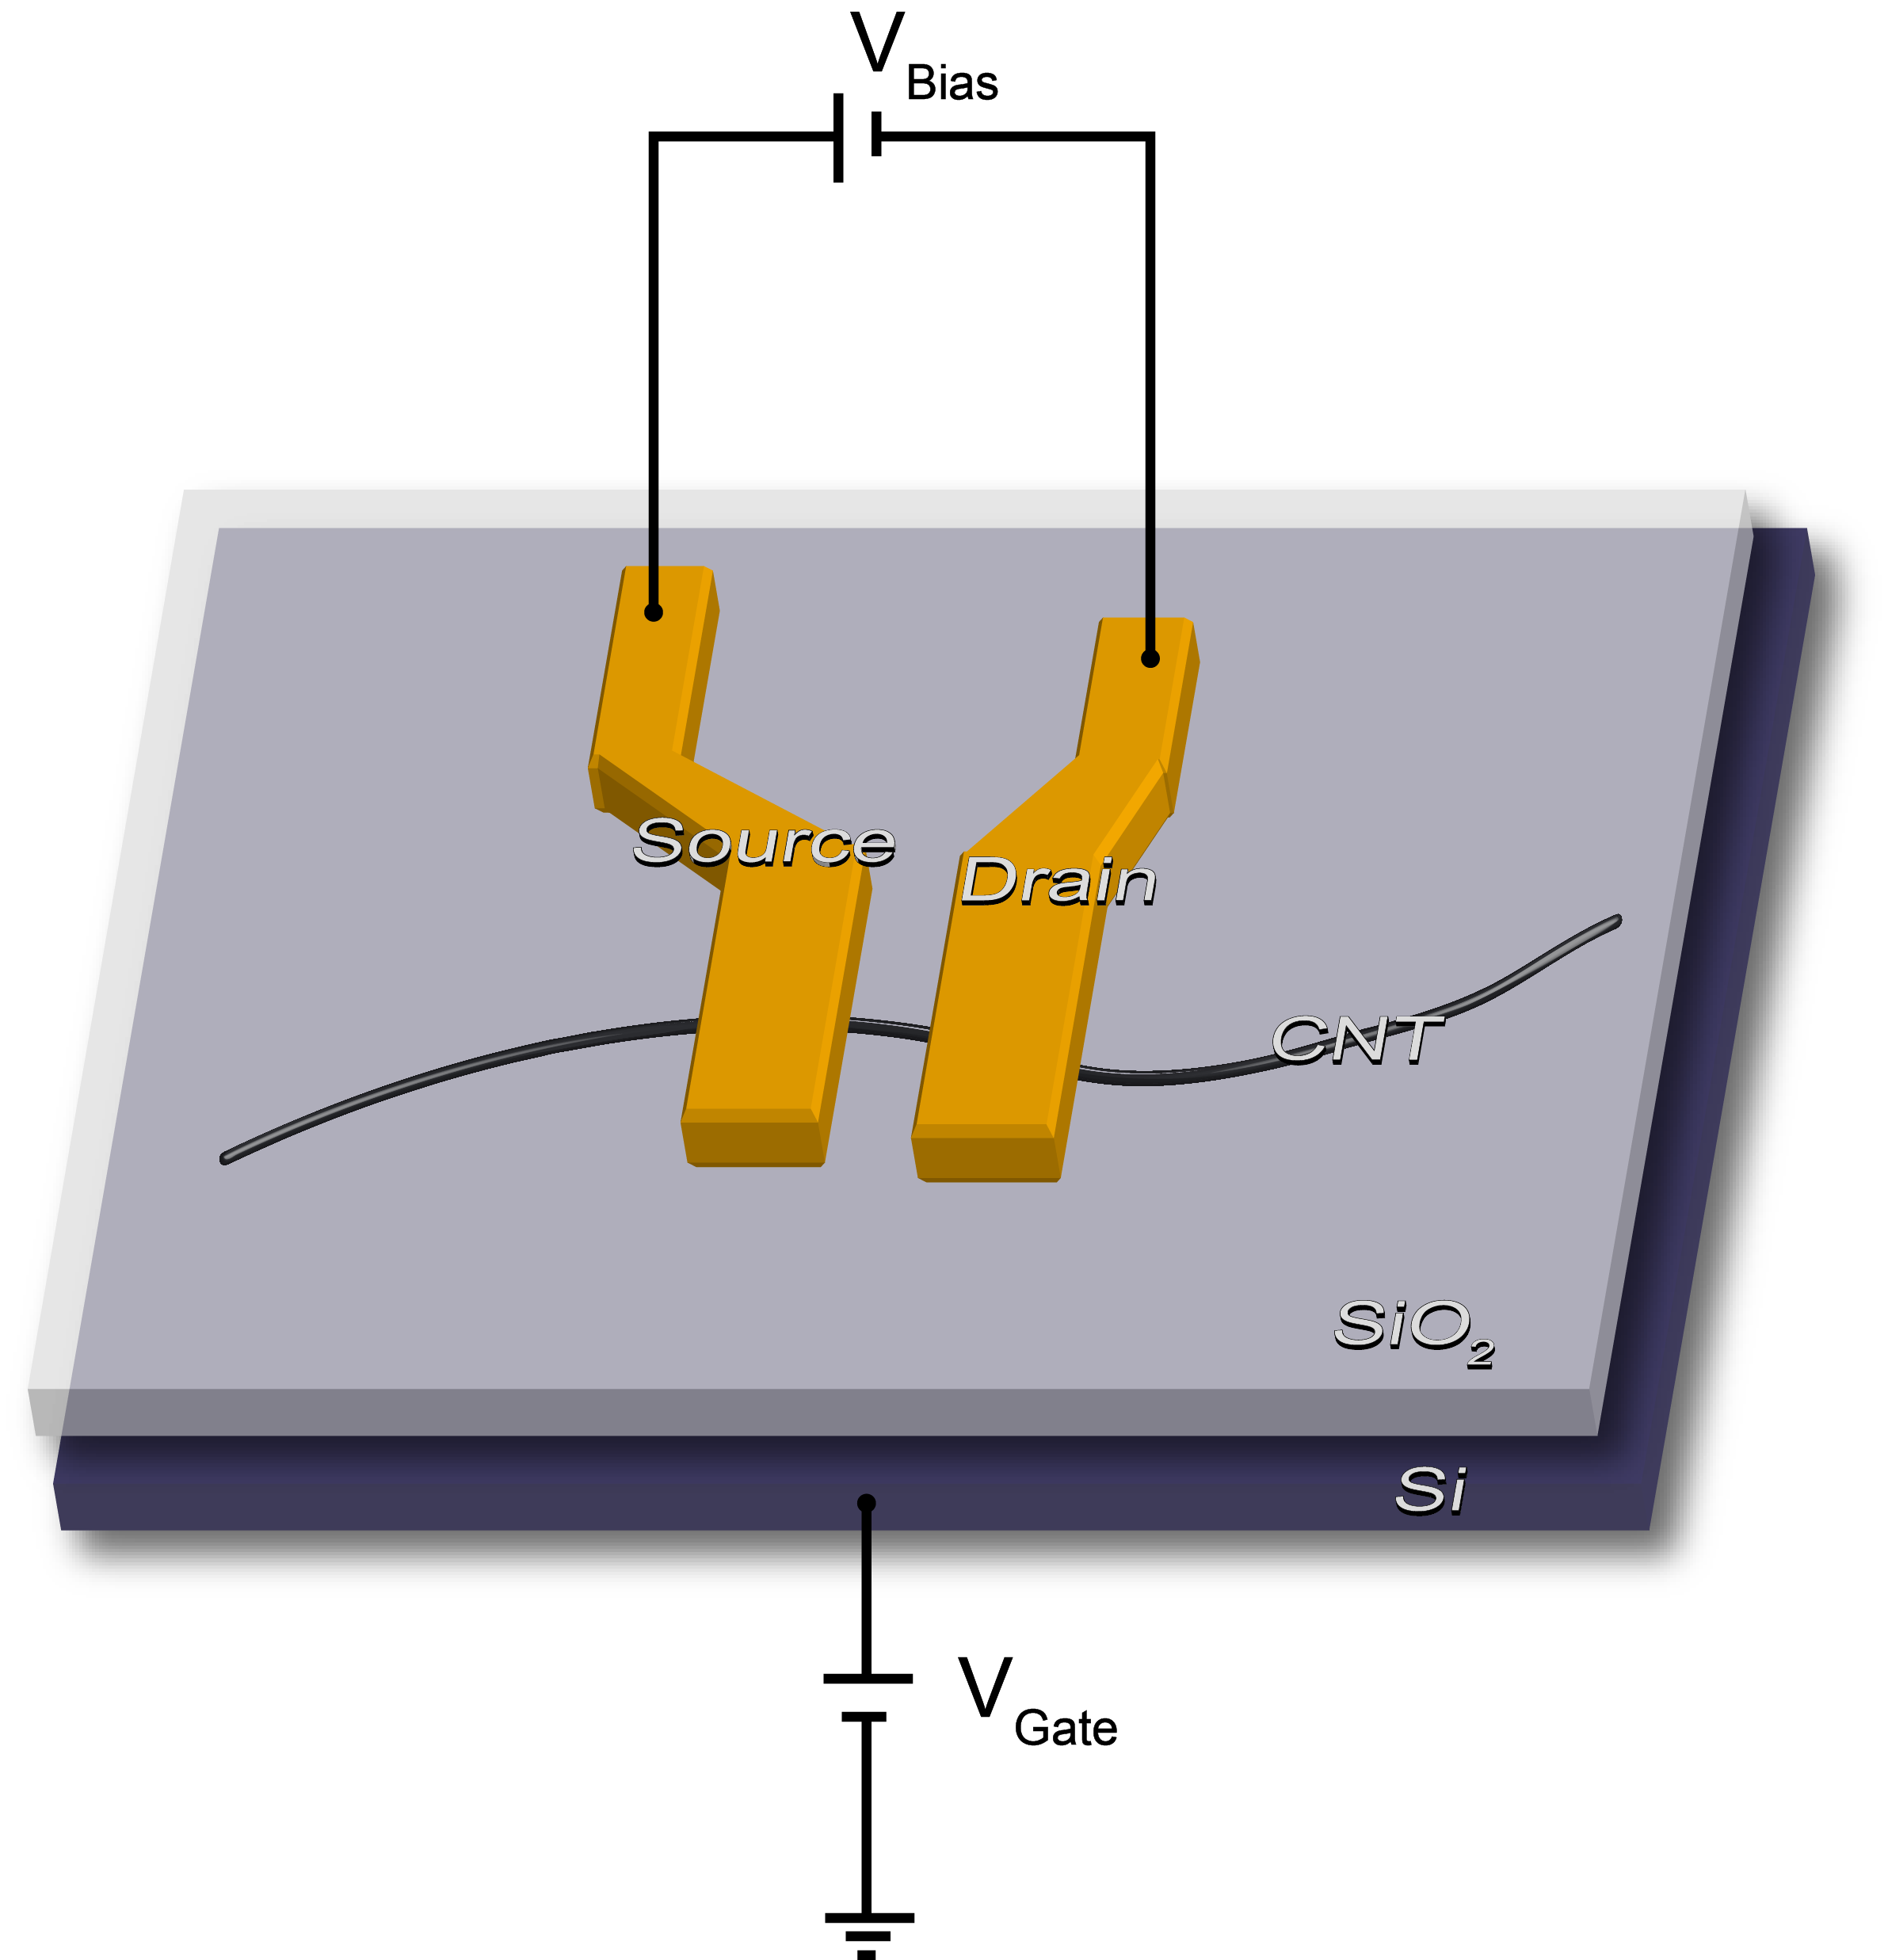
\includegraphics[width = 0.5\textwidth]{chapter2/nanotube_FET_device.png}
    \caption{Schematic of a carbon nanotube field effect transistor.}
    \label{fig:nanotube_fet}
\end{figure}

Measurements on carbon nanotube field effect transistors (CNTFETs) depend on the type of carbon nanotube that has been contacted.

\begin{figure}
    \centering
    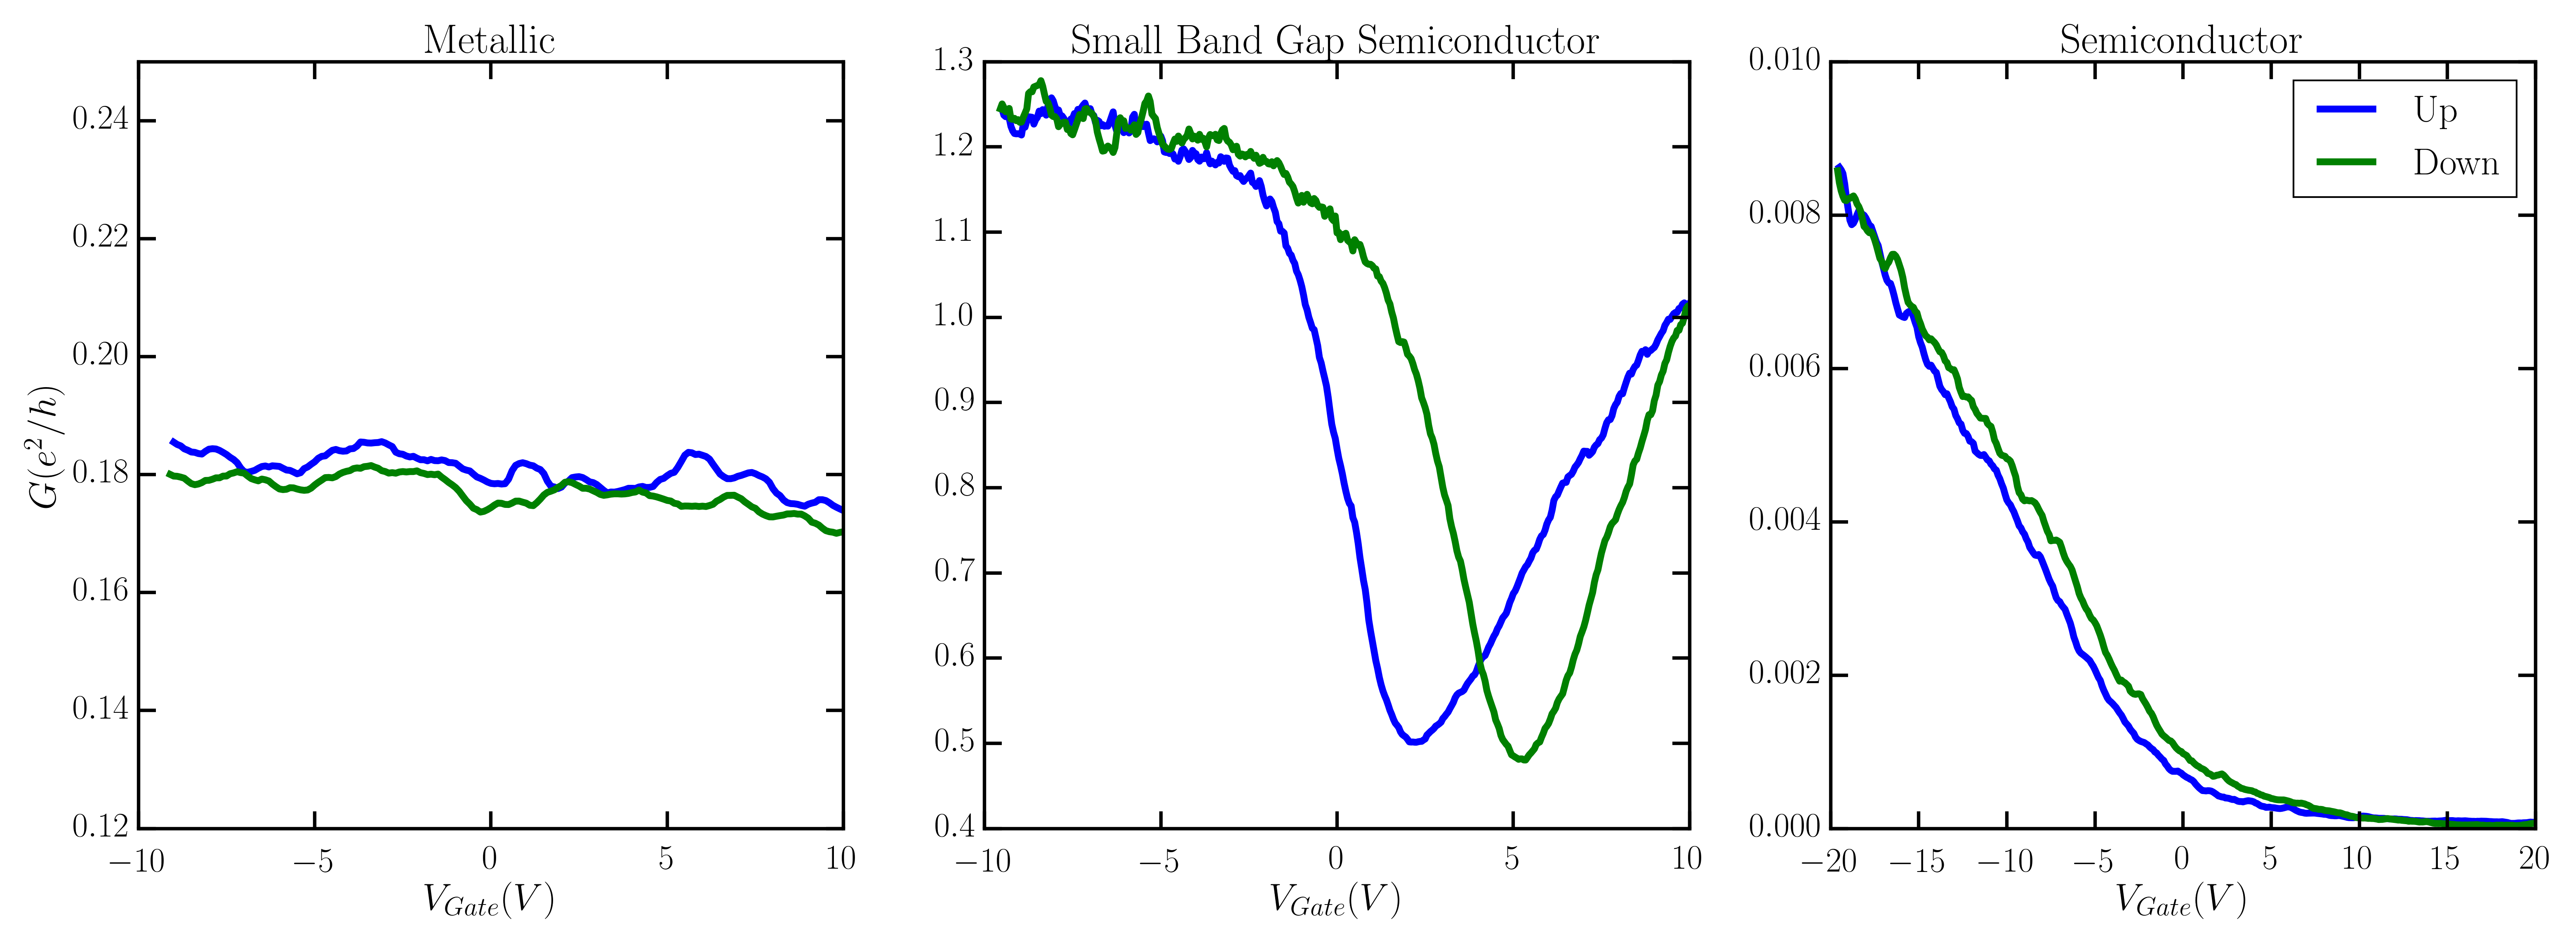
\includegraphics[width=1.0\textwidth]{chapter2/fet_measurements.png}
    \caption{Current versus gate voltage characteristics for three typs of CNTFET.}
    \label{fig:fet_measurements}
\end{figure}

\begin{figure}
    \centering
    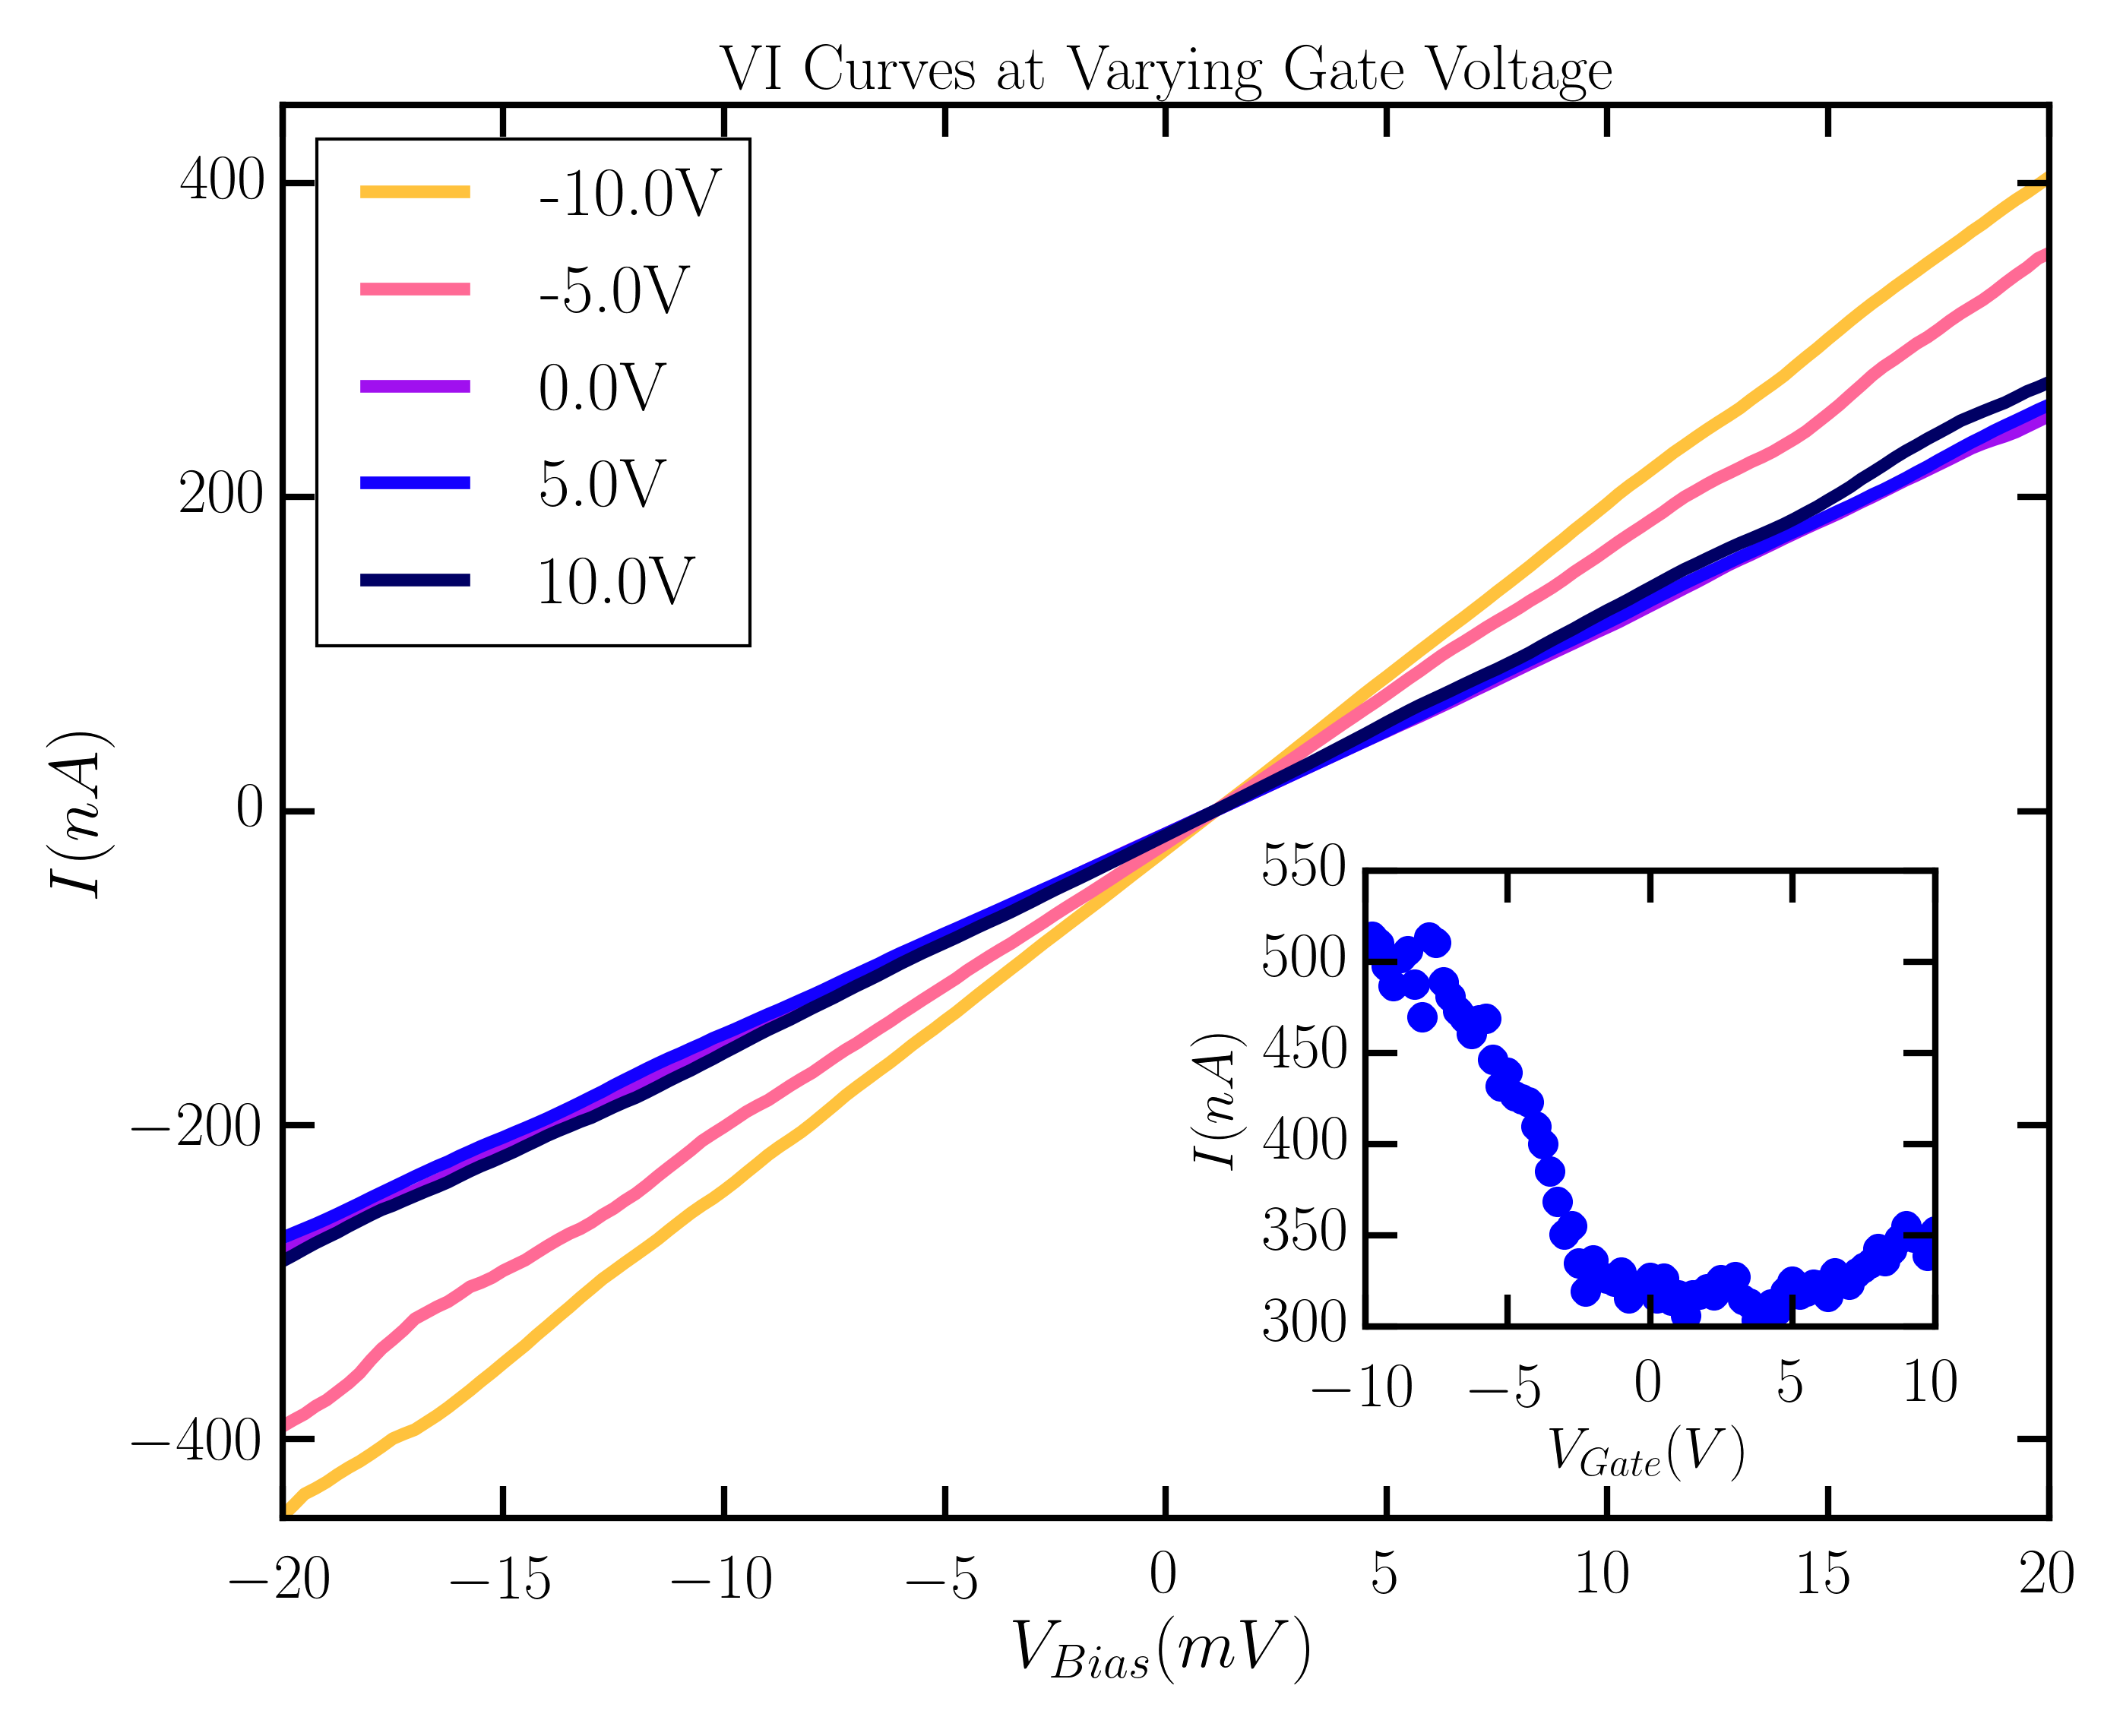
\includegraphics[width=0.7\textwidth]{chapter2/transistor_curves.png}
    \caption{IV characteristics of a typical small band gap semiconducting CNTFET. The current saturates at higher bias voltage, but is not typically measured due to avalanche breakdown of the devices. Inset: Current versus gate at a fixed bias for the same device.}
    \label{transistor_curves.png}
\end{figure}

Metallic source/drain contacts typically form Schottky barriers with carbon nanotubes. The polarity of the resulting CNTFET is thus determined by the relation between the work function of the contact material and nanotube. For metals with a relatively high work function, such as Pd, Ti, Cr, and Co, the devices are expected to be p-type. Metals with a lower work function, such as Al, Mg, and Sc, can produce n-type transistors. However, many of these low work function metals also happen to have a very poor wetability on the nanotube surface, which leads to large contact resistances, making the devices very difficult to fabricate and measure.

\section{Carbon Nanotube Quantum Dots}

When cooled to low temperatures ($\lesssim \SI{10}{\kelvin}$), the device drawn in Figure \ref{fig:nanotube_fet} exhibits quantum mechanical behavior. For a sufficiently short channel length ($L \lesssim \SI{500}{\nano\meter}$), electrons become confined within the carbon nanotube and behave like quantum mechanical particles in a box. This device is called a quantum dot. The resistance versus temperature plot in Figure \ref{fig:CNT_RT} shows the sharp increase in resistance as the tunneling through the device is suppressed at low temperatures. 

\begin{figure}
    \centering
    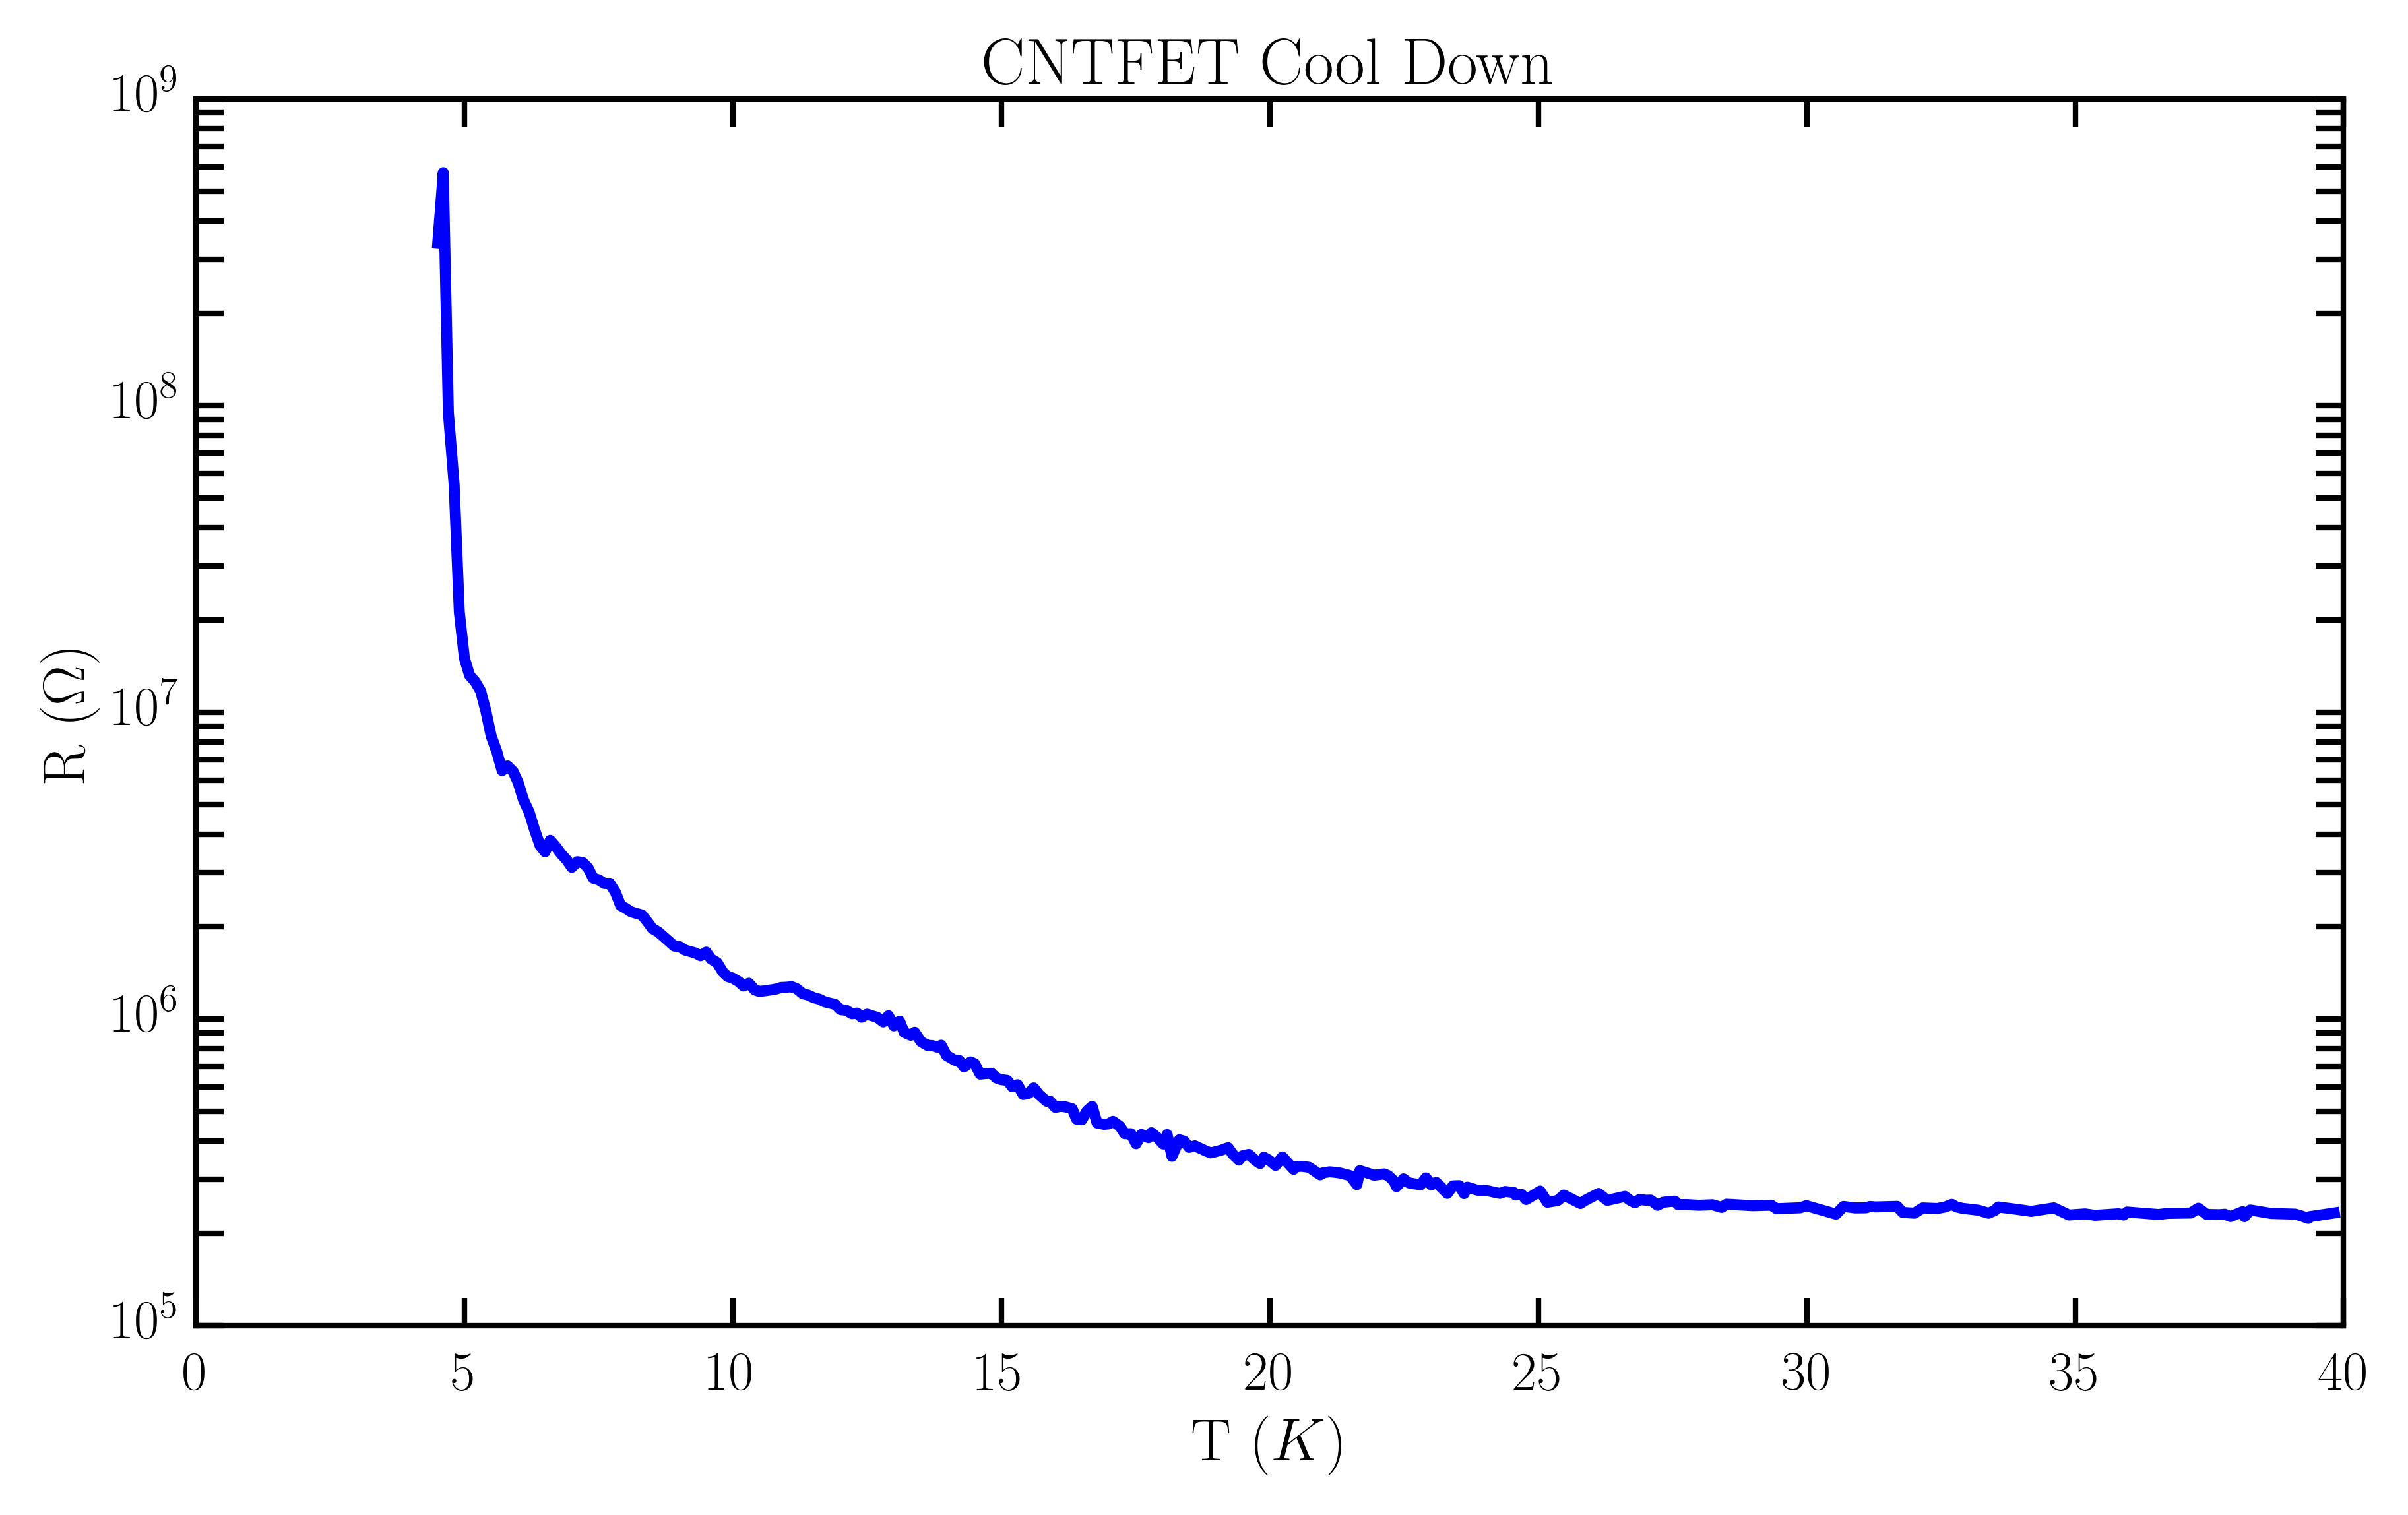
\includegraphics[width=0.6\textwidth]{chapter2/cntfet_cooldown.png}
    \caption{R-T curve of a CNTFET cooled to \SI{4}{\kelvin}}
    \label{fig:CNT_RT}
\end{figure}

Once the device is cold, the filling of electrons can be controlled by varying the bias and gate voltages. A schematic of the relevant energies is seen in Figure \ref{fig:QD_model}. The bias voltage can be used to change the relative chemical potential of the source and drain metals. The gate voltage is then used to change the chemical potential on the quantum dot relative to the source/drain.

\begin{figure}
    \centering
    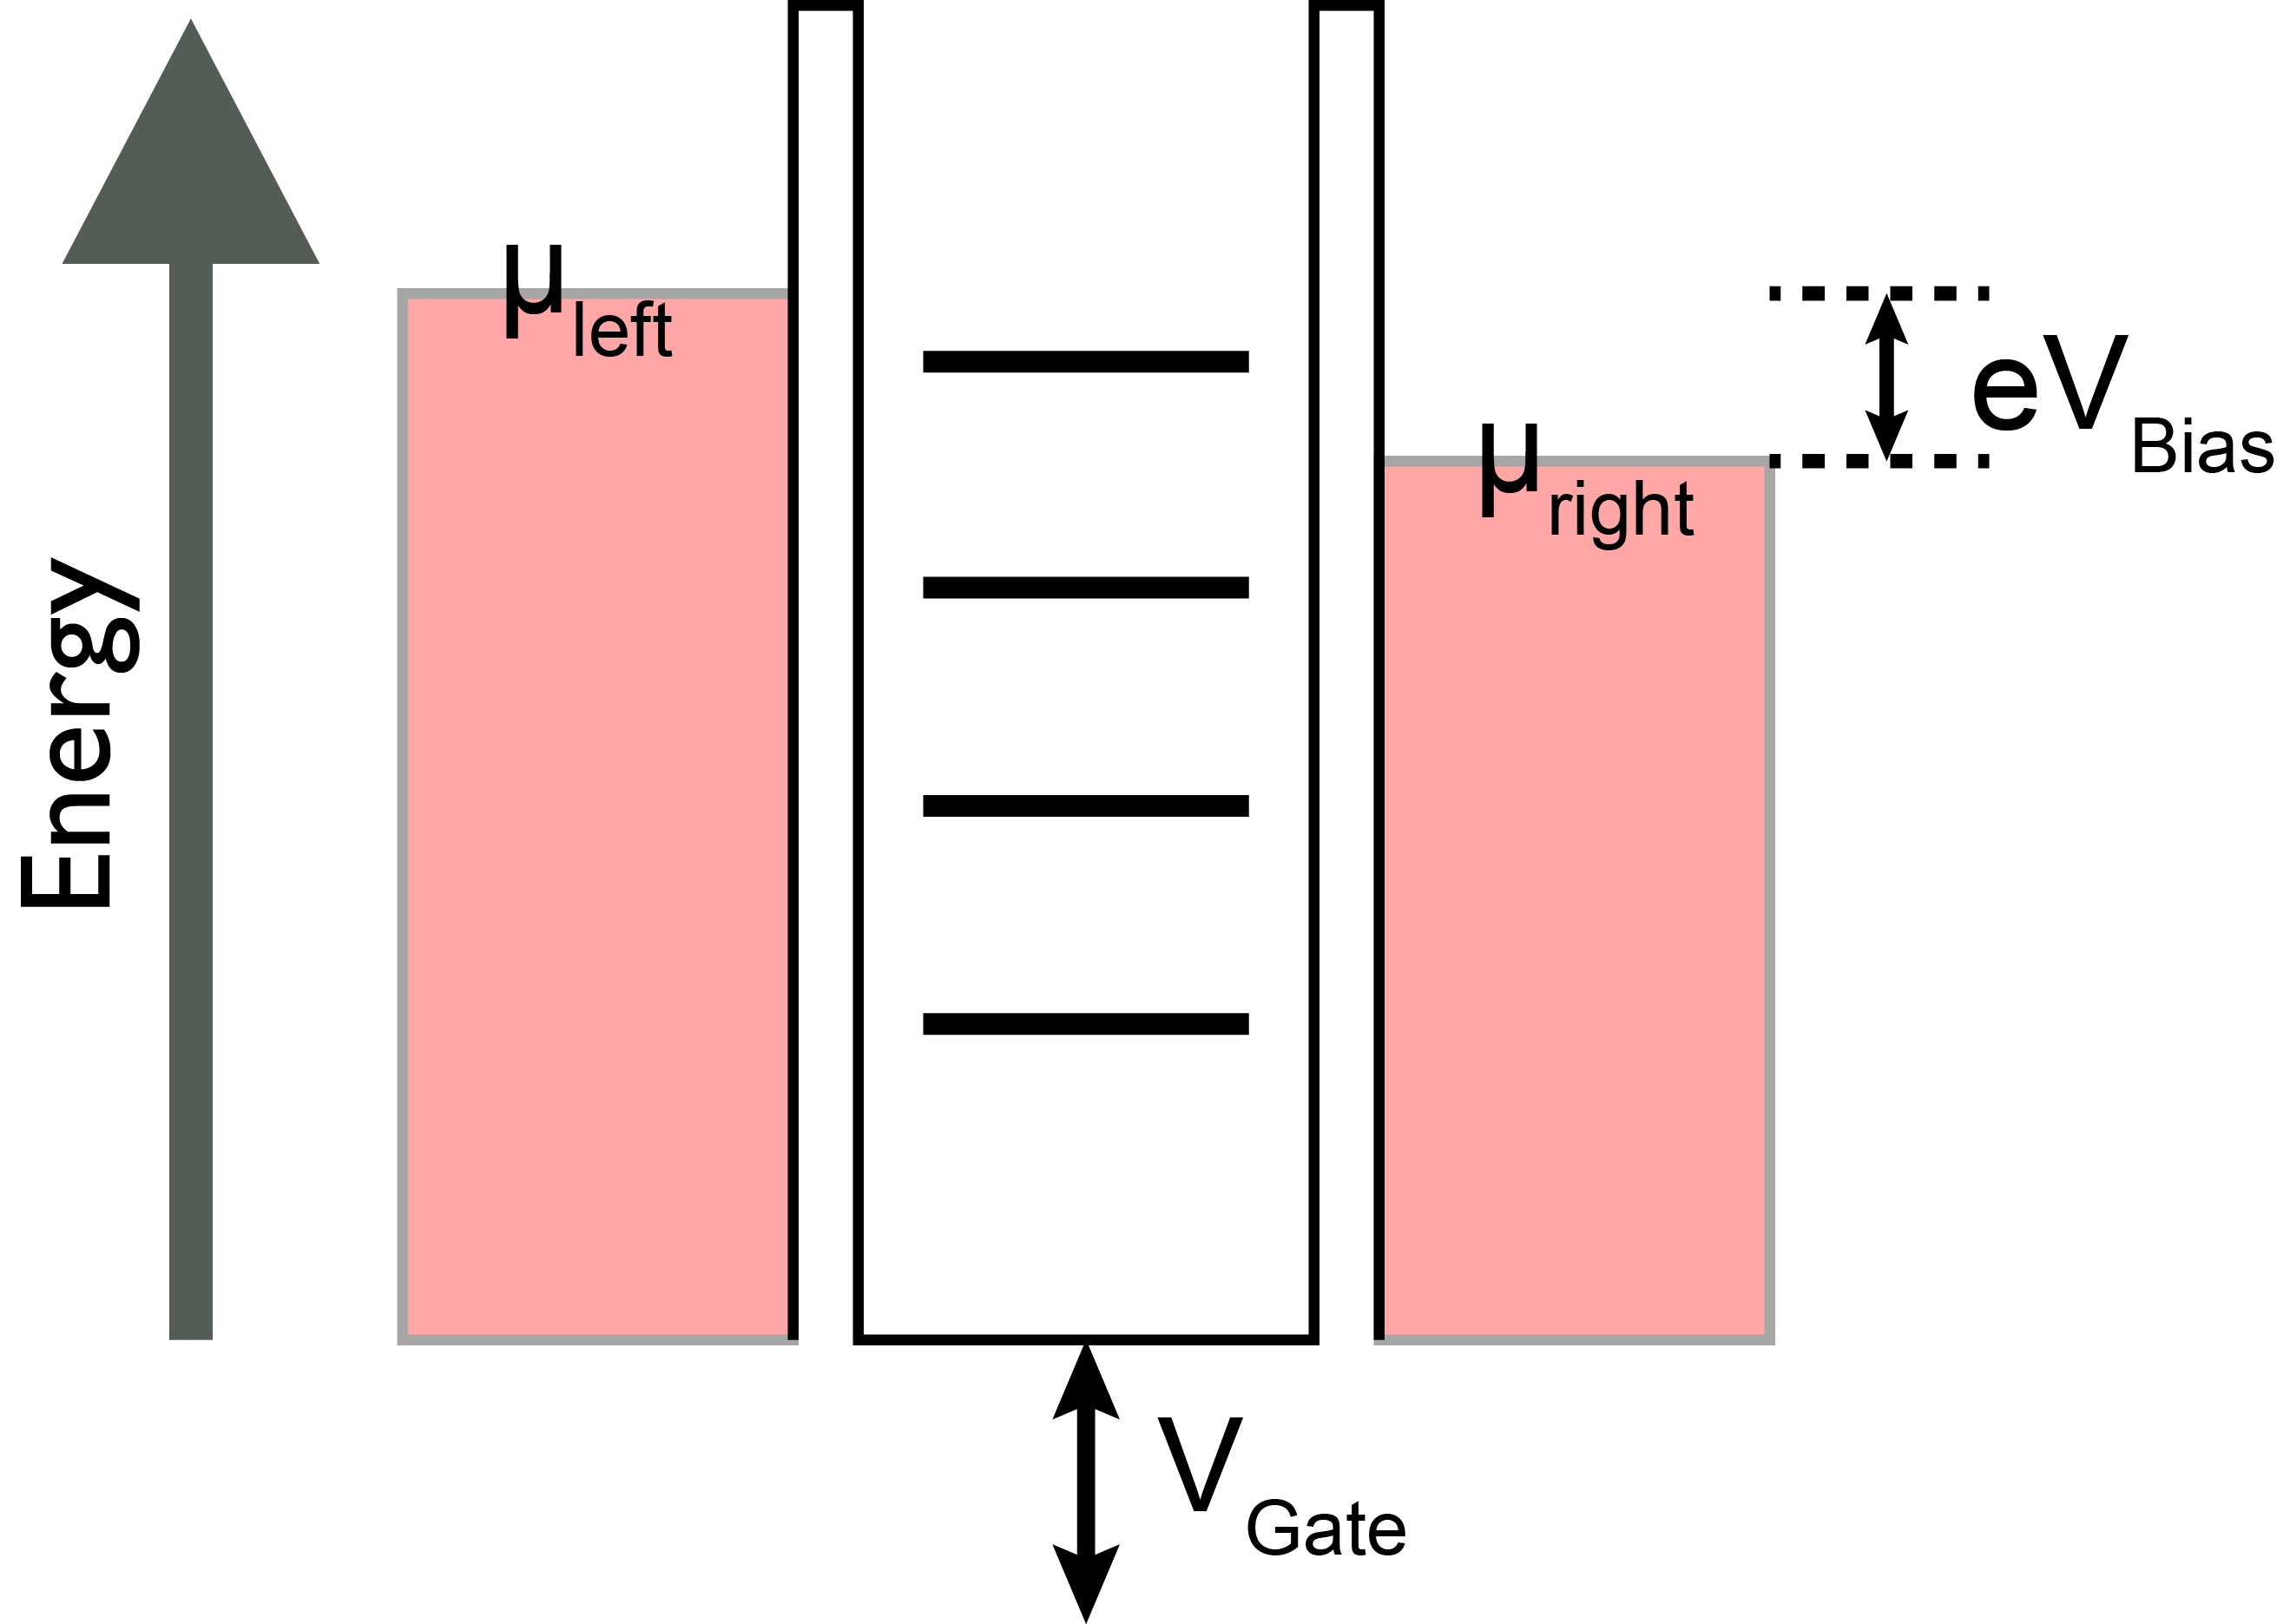
\includegraphics[width=0.5\textwidth]{chapter2/quantum_dot_model.png}
    \caption{Quantum dot energy diagram.}
    \label{fig:QD_model}
\end{figure}

The model we will use to discuss this device is called the constant interaction model. Tunnel barriers naturally form at the interface between the metal contacts and the nanotube. At low temperatures this leads to weak tunneling on/off the nanotube (quantum dot). Because of this, the number of electrons confined on the dot at any given time is an integer, N. Adding an additional electron to the dot requires overcoming the Coulomb repulsion between the additional electron and those already confined on the dot. The constant interaction model treats this charging energy as a constant, regardless of the number of electrons confined on the dot. The model also assumes that the states on the quantum dot are not affected by the electron-electron interactions.

With these assumptions, it is simple to find the energy required to add an electron to the dot. To begin, the total energy on the dot can be approximated.

\begin{equation}
    U(N) = \frac{[e(N-N_0) - C_gV_g]^2}{2C} + \sum_{N}^{} E_n
\end{equation}

Here $N_0$ is the charge on the dot a zero gate voltage, $C_g$ is the gate capacitance, and $C = C_source + C_drain + C_gate$. The summation represents the sum over all of the filled quantum dot leves, denoted by $E_n$. The chemical potential is defined as $\mu(N) = U(N) - U(N+1)$. 

\begin{equation}
    \mu(N) = (N - N_0 - \frac{1}{2})\frac{e^2}{2C} - \frac{eC_gV_g}{C} + E_N
\end{equation}

Finally, the addition energy is given by the change in chemical potential from the $N$ to $N+1$ levels.

\begin{align}
    \Delta \mu(N) &= \frac{e^2}{2C} + (E_N+1 - E_N) \nonumber \\
    \Delta \mu(N) &= \frac{e^2}{2C} + \Delta E  \label{eq:addition_energy}
\end{align}

Equation \ref{eq:addition_energy} gives the amount of energy required to add the Nth electron to the quantum dot. Note that the first term in this energy is the constant interaction term representing the Coulomb repulsion, $E_{charging} = \frac{e^2}{2C}$. 

The simplest measurement to make on a quantum dot like the one described here, is to measure the conductance as a function of the gate voltage. Figure \ref{fig:gate_blockade} shows diagrammatically how the process works. At very small bias ($\mu_{left} \sim \mu_{right}$), the gate voltage is varied. When the chemical potential on the source/drain are resonant with a level on the quantum dot, a peak is observed in the conductance. Otherwise, conductance  across the dot is suppressed. Spacing between conductance peaks should follow Equation \ref{eq:addition_energy}.

\begin{figure}
    \centering
    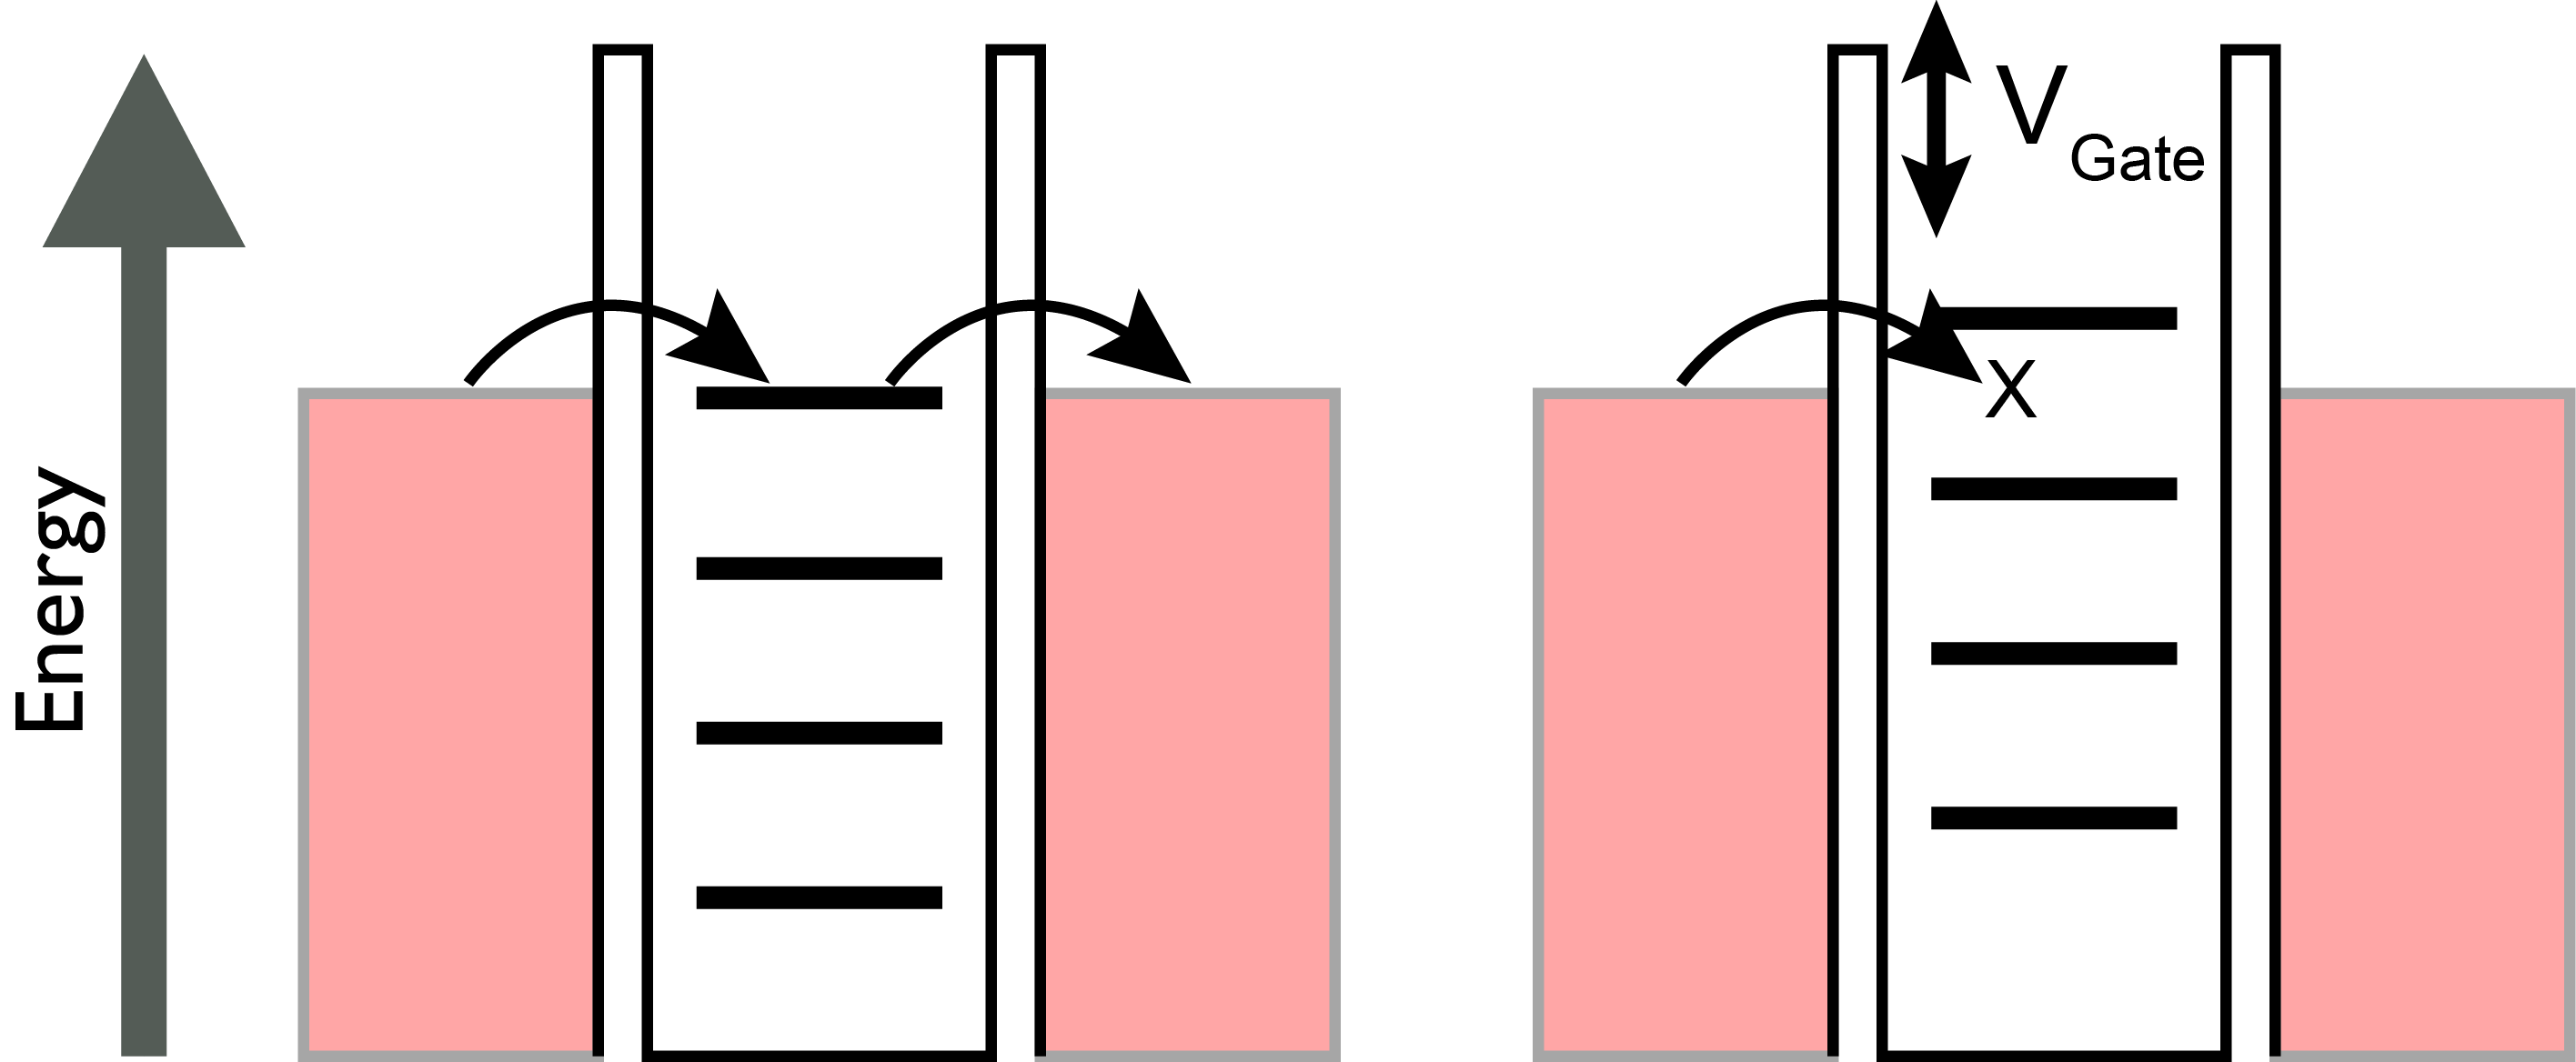
\includegraphics[width=0.8\textwidth]{chapter2/gate_blockade.png}
    \caption{Left: A quantum dot level resonant with the source/drain chemical potential. Right: The same device in the blockaded region.}
    \label{fig:gate_blockade}
\end{figure}

Figure \ref{fig:real_gate} shows conductance as a function of gate voltage through an actual carbon nanotube quantum dot device. A close look at the spacing of the conductance peaks reveals some hints of four-fold symmetry that is an important part of the structure of the nanotube quantum dot. Addinzag the first electron to the dot costs an energy $ \Delta \mu(N) = \frac{e^2}{2C} + \Delta E$. However, the electron spin and valley degeneracy combine to give each level in the quantum potential well a degeneracy of four. The next three electrons added move into the same level, which only requires an energy of $\Delta \mu(N) = \frac{e^2}{2C}$ for each electron. This pattern continues for each level on the dot, such that the energy required to add the $N$ electron is always larger than the energy required to add the $N+1$, $N+2$, and $N+3$ electrons.

\begin{figure}
    \centering
    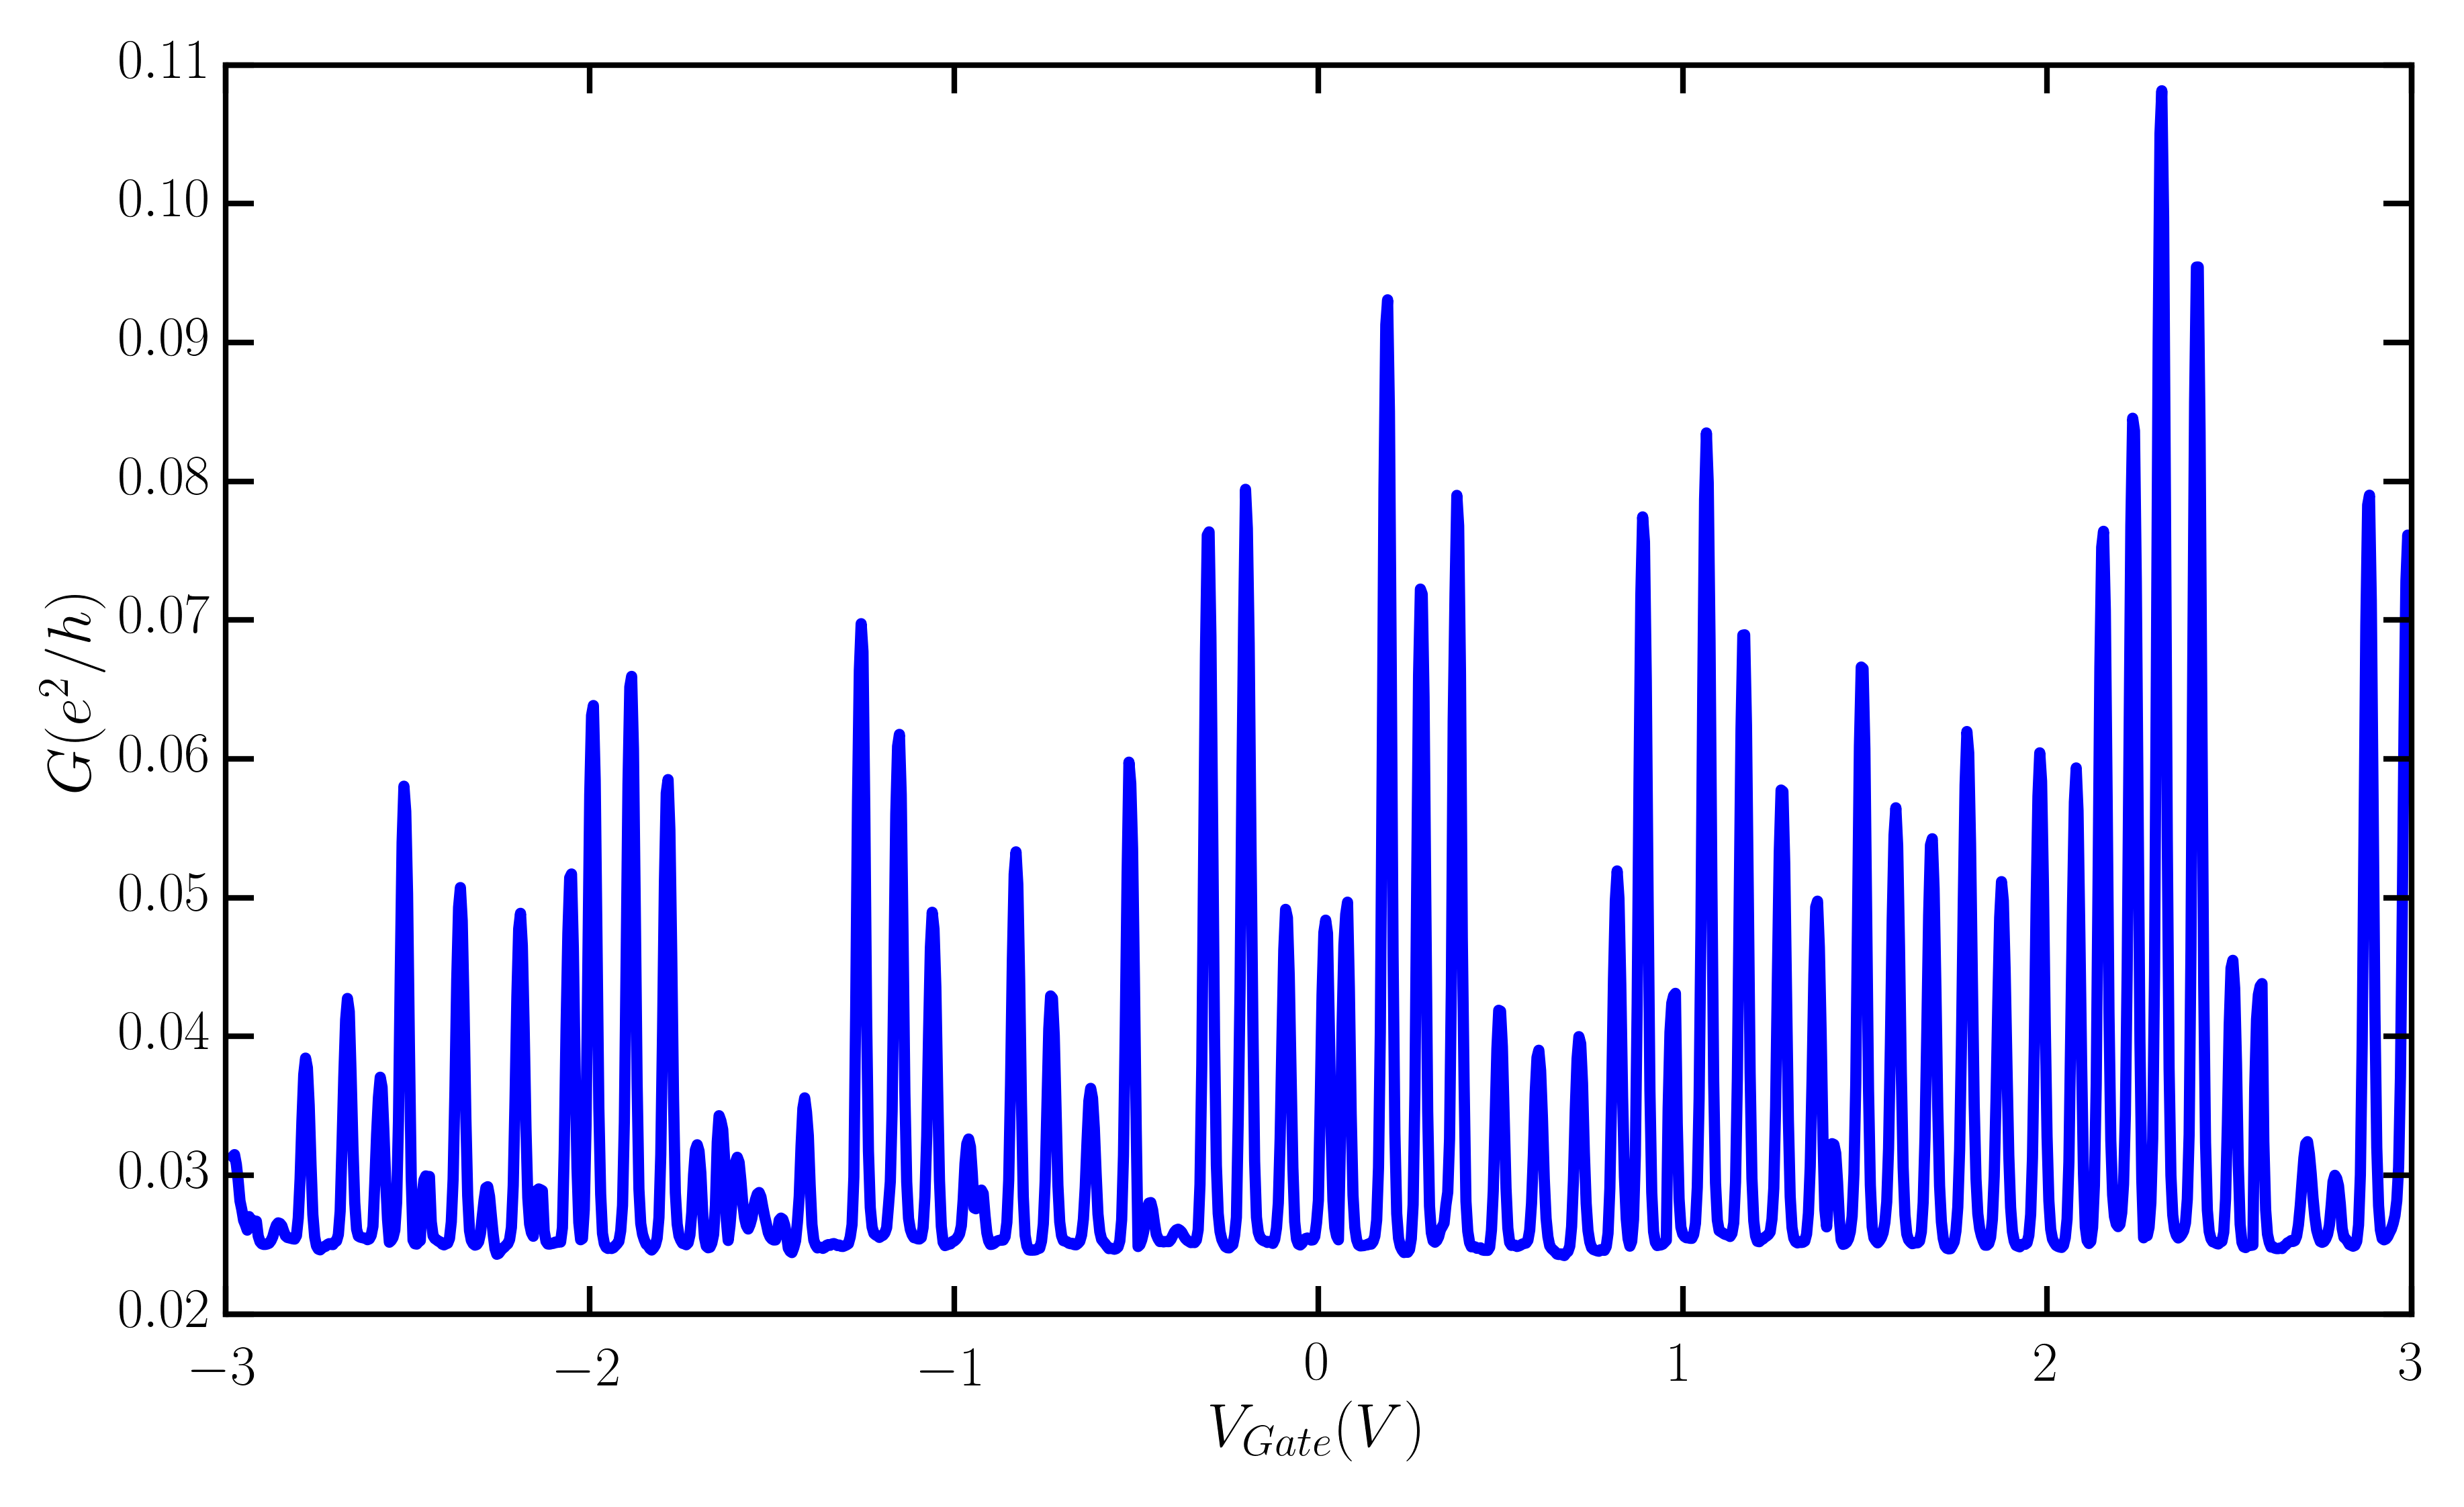
\includegraphics[width=0.8\textwidth]{chapter2/gate_sweep.png}
    \caption{Conductance as a function of applied gate voltage in a cobalt contacted nanotube quantum dot.}
    \label{fig:real_gate}
\end{figure}

Varying the bias voltage leads to similar behavior, as illustrated in Figure \ref{fig:bias_blockade}. If a level on the quantum dot lies between the source and drain chemical potentials, conductance is possible. Otherwise, if no level lies in that window, the device is again in the blockaded regime. With further increases of the bias voltage, higher order conductance processes are possible. 

\begin{figure}
    \centering
    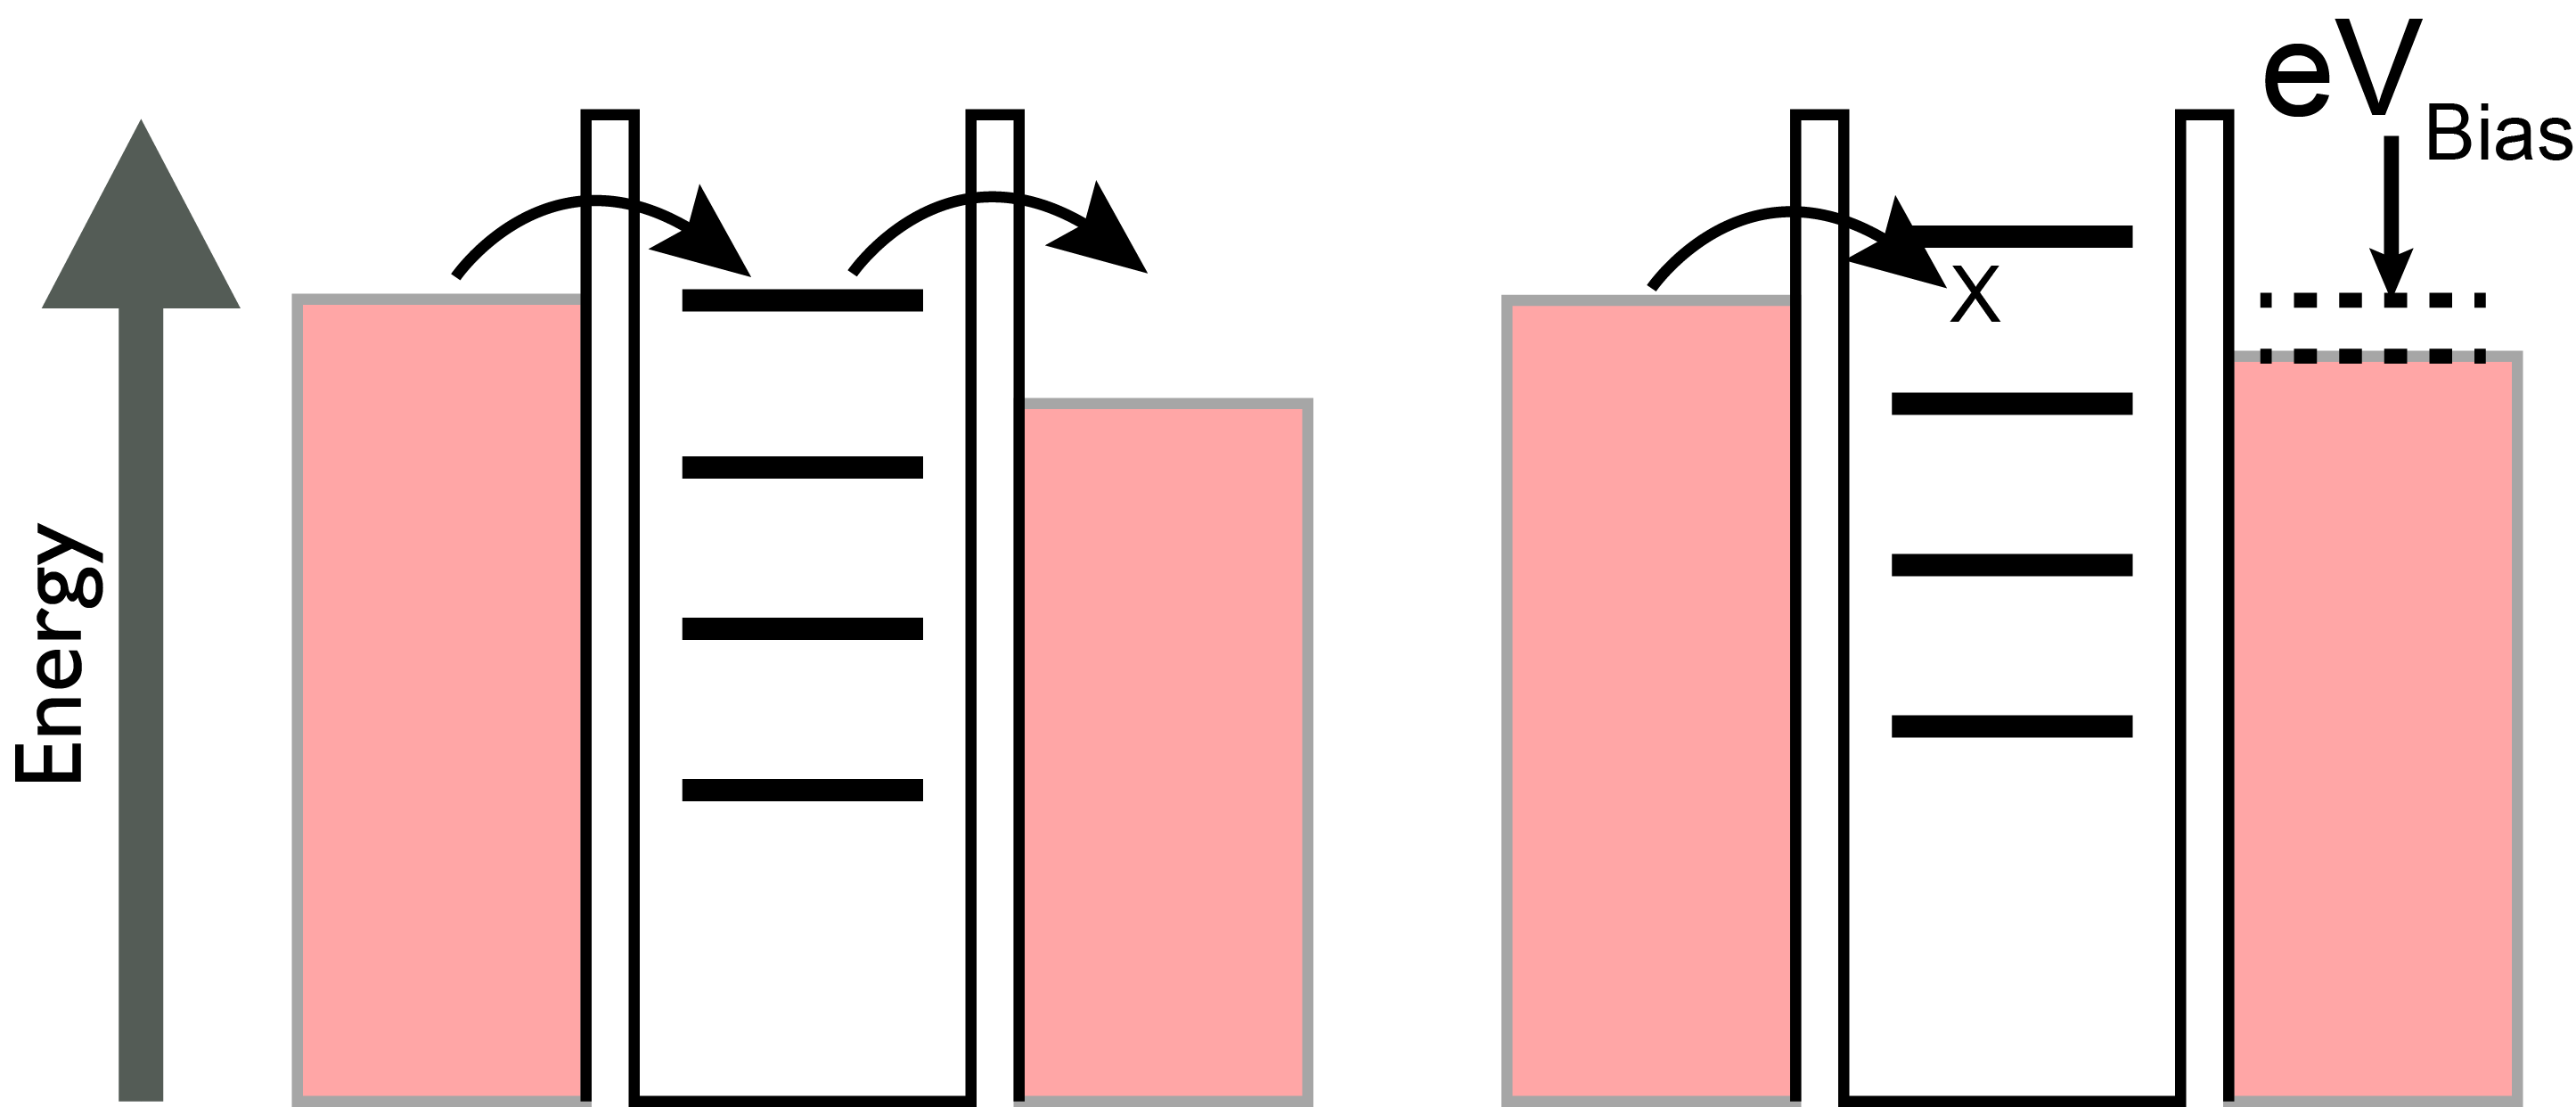
\includegraphics[width=0.8\textwidth]{chapter2/bias_blockade.png}
    \caption{Left: A quantum dot level resonant with the drain chemical potential. Right: The same device in the blockaded region.}
    \label{fig:bias_blockade}
\end{figure}

\begin{figure}
    \centering
    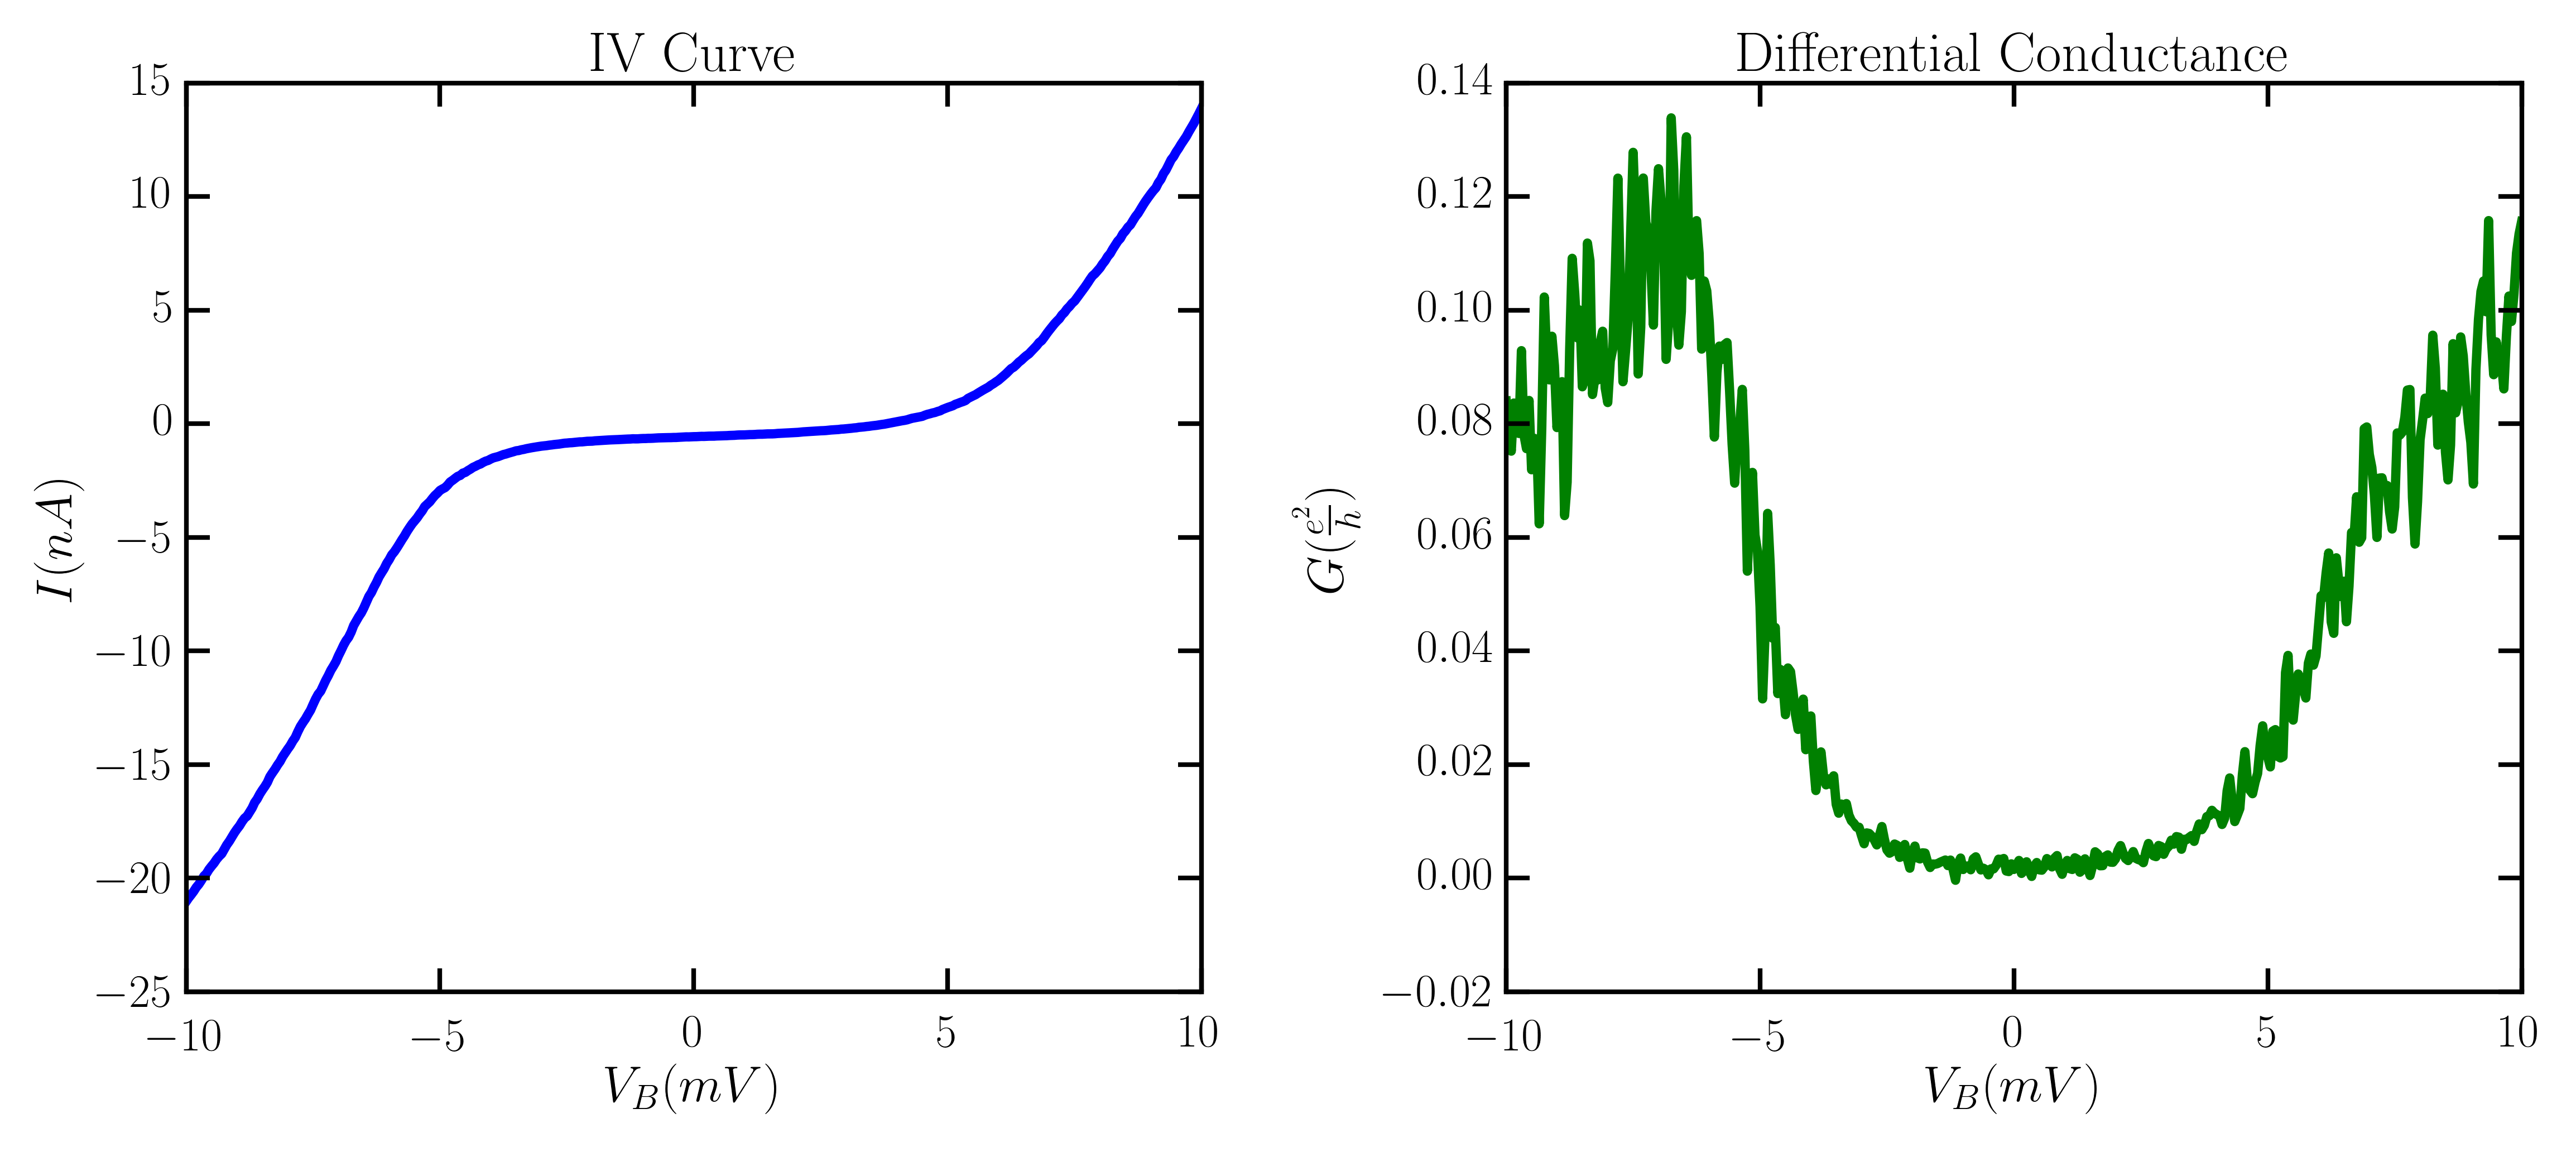
\includegraphics[width=0.8\textwidth]{chapter2/bias_sweep.png}
    \caption{Left: An IV curve at fixed gate voltage Right: Differential conductance measured at fixed gate voltage.}
    \label{fig:real_bias}
\end{figure}

Figure \ref{fig:real_bias} shows current and conductance as a function of applied bias voltage. It is clear from the differential conductance plot, for low bias voltages the conductance is suppressed across the dot. At higher bias, a quantum dot level moves into the bias window and conductance increases. Increasing the bias further from there allows for transport through excited states and higher order processes, which will be discussed further in later chapters.

Finally, measuring conductance as a function of both the bias and gate produces a stability diagram of the quantum dot. An example of this can be seen in Figure \ref{fig:coulomb_diamonds}. Looking at a cut of this plot at constant bias reproduces Figure \ref{fig:real_gate}. Similarly, a cut at constant gate voltage reproduces Figure \ref{fig:real_bias}. Putting both together produces diamond-shaped regions in which the charge on the quantum dot in constant, denoted by $N-1$, $N$, and $N+1$ in the figure. The white dashed lines serve as a guide to the eye. The two black arrows mark the level spacing, $\Delta E$, and addition energy $E_Add$ (or $\Delta \mu$). By measuring both of these quantities it is possible to know the level spacing on the quantum dot and the capacitance of the device. By observing changes in the conductance peaks at different fillings and applied fields much can be learned about the levels on, interactions in, and transport across the quantum dot.

\begin{figure}
    \centering
    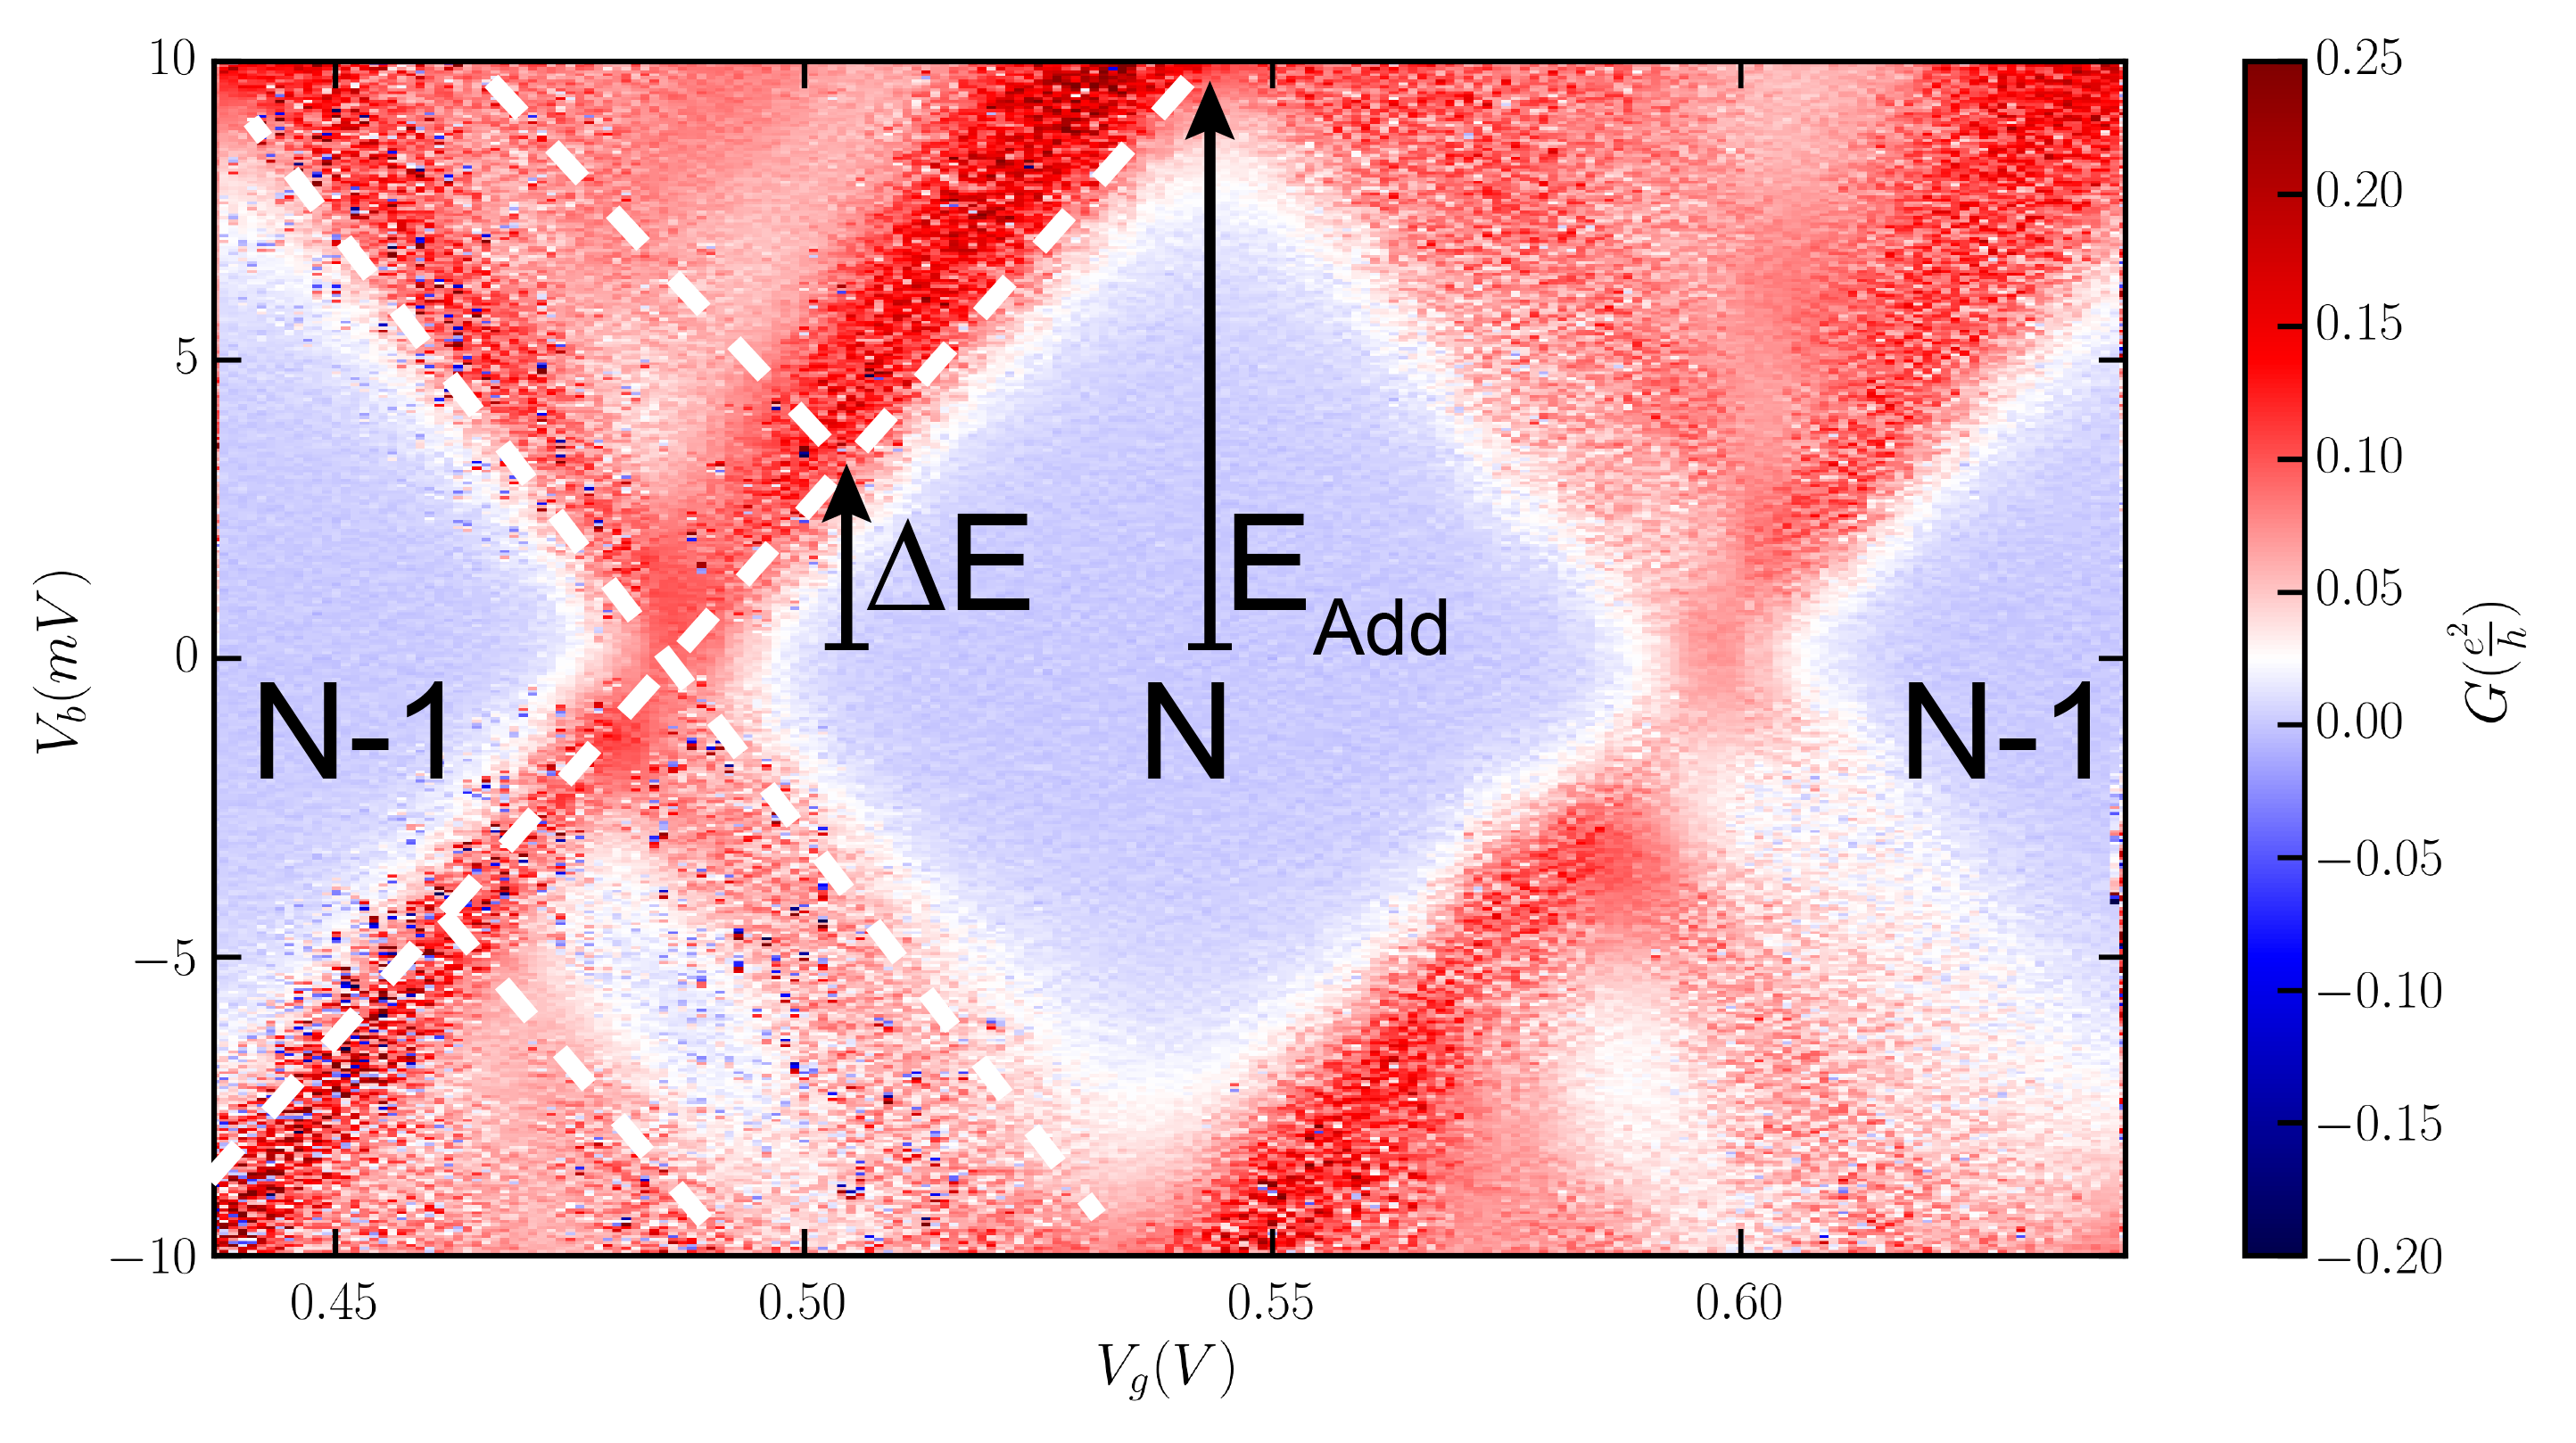
\includegraphics[width=0.7\textwidth]{chapter2/diamond_diagram.png}
    \caption{Conductance of a cobalt contacted nanotube quantum dot at 4K as a function of bias and gate voltages.}
    \label{fig:coulomb_diamonds}
\end{figure}